%%%%%%%%%%%%%%%%%%%%%%%%%%%%%%%%%%%%%%%%%%%%%%%%%%%%%%%%%%%%%%%%%%%%%%%%%%%
%%  chapter2.tex  –  Глава 2: Методы, алгоритмы и математические
%%                   основы для робастных динамических графовых нейронных сетей
%%  v9 – Единая постановка задачи с последовательным выводом.
%%       Декомпозиция на 7 подзадач, сопоставленных пробелам.
%%       Все доказательства, алгоритмы и анализ сложности сохранены.
%%       Только заголовки \section добавлены в оглавление.
%%%%%%%%%%%%%%%%%%%%%%%%%%%%%%%%%%%%%%%%%%%%%%%%%%%%%%%%%%%%%%%%%%%%%%%%%%%

\chapter{Математическая модель гибридная СОПВ и предлагаемые модели и алгоритмы повышения её робастности и эффективности}
\label{ch:methods}

Глава разрабатывает теоретическое ядро: \S\ref{sec:hybrid_idps_math_model} формализует гибридную СОПВ и ставит шесть сквозных свойств П1--П6 как исследовательские вопросы с инвариантами; \S\ref{sec:unified_problem} формулирует единую задачу их совместной оптимизации; разделы \ref{sec:ct_tgnn}--\ref{sec:game} представляют семь моделей М1--М7, каждая из которых закрывает инварианты из табл.~\ref{tab:six_properties}; \S\ref{sec:metrics_taxonomy} систематизирует 23 метрики оценки качества по шести свойствам.
%%====
\section*{Соглашения об обозначениях}
\label{sec:notation_conventions}
\addcontentsline{toc}{section}{Соглашения об обозначениях}
%%====

В рамках всей диссертации перечисленные ниже символы используются
\emph{единообразно}; локальные переопределения допускаются только при
явном указании в тексте.

\begin{itemize}[leftmargin=2em, itemsep=0pt]

\item $f_\theta$~--- \emph{обучаемый детектор} гибридная СОПВ,
параметризованный вектором $\theta\in\Theta$, отображающий
наблюдения в момент~$t$ в распределение вероятностей по классам
угроз: $f_\theta:(X_t,A_t)\mapsto \hat y_t\in\Delta^{K}$. \emph{В
сертифицированных архитектурах} (модели~М1, М3) $f_\theta$
дополнительно выступает в роли правой части нейронного
обыкновенного дифференциального уравнения, описывающего эволюцию
скрытых представлений: $\dot{\bh}_v(t)=f_\theta(\bh_v(t),A(t),t)$;
в этом случае подразумевается \emph{одна и та же} семья функций,
ограниченная по Липшицу с константой~$L_g$. Никакая другая
функция в тексте символом~$f_\theta$ не обозначается.

\item $g_\psi$~--- \emph{модуль реагирования}
(response/policy mapping), параметризованный вектором~$\psi$,
отображающий апостериорные оценки и контекст в действие
$a\in\calA$: $g_\psi:(\hat y_t,\,c_t)\mapsto a_t$. Применяется в
теоретико-игровом блоке М7 и в RL-агентах. Символом~$g$ без
индекса~$\psi$ обозначается векторное поле нейронного ОДУ
(когда требуется отделить его от детектора), что оговаривается
локально.

\item $\pi$~--- \emph{политика} распределения действий
(в смысле RL/Stackelberg): $\pi(a\mid s)$. Не путать с числом
$\pi$ в тригонометрических контекстах, где сохраняется обычная
интерпретация.

\item $L_g$~--- \emph{константа Липшица} правой части нейронного
ОДУ~$f_\theta(\cdot,t)$ по аргументу скрытого состояния:
$\|f_\theta(\bh_1,t)-f_\theta(\bh_2,t)\|\le L_g\|\bh_1-\bh_2\|$.
$L_g$~--- ключевой параметр сертификата робастности по Грёнуоллу:
$\|\bh_1(T)-\bh_2(T)\|\le e^{L_g T}\|\bh_1(0)-\bh_2(0)\|$.
Численная оценка $\hat L_g$ выполняется методом степенной
итерации (см.~Главу~6). \emph{Защита оценки $L_g$:} оператор
свёртки на графе является композицией линейного оператора
(матрица смежности), нелинейности (Tanh/GELU с
$\mathrm{Lip}\le 1$) и обучаемой матрицы весов $W$; верхняя граница
$L_g\le \|W\|_{\mathrm{op}}\cdot \mathrm{Lip}(\sigma)\cdot
\|A\|_{\mathrm{op}}$ оценивается операторно-нормально и
эмпирически тестируется на валидационной выборке.

\item $L_c$~--- \emph{константа Липшица головы классификатора}
$h\mapsto\mathrm{logits}$. Сквозная константа Липшица отображения
вход~$\to$ логиты равна $L_c\cdot e^{L_g T}$; сертифицированный
радиус робастности по~$\ell_2$:
$\rho=\Delta_{\min}/(L_c\,e^{L_g T})$, где $\Delta_{\min}$~---
запас между двумя наибольшими логитами.

\item $L_a$~--- \emph{константа Липшица механизма внимания}
(M3, TripleE-TGNN). Для softmax-внимания с обучаемыми
$Q,K,V\in\R^{d\times d}$: $L_a\le
\|V\|_{\mathrm{op}}\cdot 4\,d^{1/2}\cdot
\|Q\|_{\mathrm{op}}\|K\|_{\mathrm{op}}$ (Kim et al., 2021).
Использование $L_a$ требуется для распространения границ
сертифицированной робастности на блоки внимания: сквозная
константа модели становится $L_c\cdot L_a\cdot e^{L_g T}$,
что усиливает требование к спектральной норме весов внимания
$\|Q\|_{\mathrm{op}}\|K\|_{\mathrm{op}}\le 1$.

\item $\calL_g(\theta;\calG_g)$~--- \emph{потеря на уровне
гранулярности~$g$} (graph-level loss), где $g\in\{s,r,n\}$
обозначает уровень сервиса~/ трассировки~/ узла. Индекс~$g$
здесь является \emph{меткой уровня}, не путать с константой
Липшица~$L_g$ и с векторным полем~$g$.

\item $\rho$~--- сертифицированный \emph{радиус робастности}
по норме~$\ell_2$ или \emph{мощность множества} в зависимости
от контекста (с явным указанием).

\item $\delta_X$, $\Delta_A$~--- допустимое \emph{возмущение
признаков узлов} и \emph{бинарное возмущение рёбер} в
$\ell_2$- и $\ell_0$-нормах соответственно; объединяются в
угрозовом множестве $\Theta_{\mathrm{adv}}$.

\end{itemize}

\noindent Все остальные обозначения вводятся локально и
сохраняют интерпретацию в пределах своего подраздела.
%%====
\section{Формализация гибридной системы обнаружения и предотвращения вторжений}
\label{sec:hybrid_idps_math_model}
%%====

\subsection{Формальная модель гибридная СОПВ}
\label{subsec:idps_formal_model}

гибридная СОПВ как объект исследования (см.~\S\ref{sec:hybrid_idps_object})
формально описывается семёркой
\begin{equation}
\mathcal{H} \;=\; \bigl(\mathcal{V}_t,\,\mathcal{E}_t,\,X_t,\,A_t,\,
f_\theta,\,g_\psi,\,\pi\bigr),
\label{eq:hybrid_idps_tuple}
\end{equation}где компоненты системы интерпретируются следующим образом.

\noindent\textbf{$\mathcal{V}_t$}~--- множество наблюдаемых сущностей (хостов NIDS, бортовых сенсоров UAV, счетов финтех, медицинских устройств).

\noindent\textbf{$\mathcal{E}_t$}~--- множество связей: сетевых потоков, командно-телеметрических каналов, транзакций, обращений к ЭМЗ.

\noindent\textbf{$X_t \in \R^{n\times d}$}~--- матрица признаков узлов ($n=|\mathcal{V}_t|$); $d=83$ для NIDS-бенчмарков (CIC-IoT-2023, CSE-CICIDS-2018), адаптируется в других секторах.

\noindent\textbf{$A_t \in \R^{n\times n}$}~--- матрица смежности взвешенных связей.

\noindent\textbf{$f_\theta: (X_t, A_t) \mapsto \hat{y}_t \in \Delta^K$}~--- обучаемый детектор по $K$ классам ($K=34$ для NIDS, см.~Глава~\ref{ch:adaptation}).

\noindent\textbf{$g_\psi: \hat{y}_t \mapsto a_t \in \mathcal{A}$}~--- политика реагирования, выбирающая действие из $\mathcal{A}$ (оповещение, блокировка, изоляция, безопасный режим, эскалация в SOAR).

\noindent\textbf{$\pi \in \{\textsc{Passive}, \textsc{Active}, \textsc{IPS}\}$}~--- параметр режима интеграции в защитный стек.

Система работает в дискретные моменты $t=1,\dots,T$ под воздействием трёх рабочих условий: состязательной среды $(\delta_X,\Delta_A)\in\mathcal{S}_\varepsilon$ радиуса~$\varepsilon$; нестационарности $\mathcal{D}_t\neq\mathcal{D}_{t-1}$; и распределённого обучения, при котором~$\theta$ обновляется федеративно без передачи сырых данных.

\subsection{Шесть свойств гибридная СОПВ как исследовательских вопросов}
\label{subsec:six_properties}

Работа над моделью~\eqref{eq:hybrid_idps_tuple} организована вокруг шести сквозных свойств, формализованных как математические условия на компоненты семёрки и закрываемых моделями М1--М7 (см.~табл.~\ref{tab:six_properties}).

\paragraph{(П1) Состязательная устойчивость (Adversarially-resilient?).}
Детектор $f_\theta$ удовлетворяет границе чувствительности к ограниченным возмущениям:
\begin{equation}
\Bigl\|f_\theta\!\bigl(X_t+\delta_X,\,A_t+\Delta_A\bigr)
\;-\; f_\theta(X_t, A_t)\Bigr\|
\;\le\; \rho(\varepsilon),
\qquad \forall\,(\delta_X,\Delta_A)\in\mathcal{S}_\varepsilon,
\label{eq:adv_resilient_property}
\end{equation}
где $\rho(\varepsilon)\to 0$ при $\varepsilon\to 0$. Закрывается М1 (Грёнуолл, \S\ref{sec:ct_tgnn}), М4 (PAC-Байес, \S\ref{sec:mamba}), М7 (\S\ref{sec:game}).

\paragraph{(П2) Робастность (Robustness?).}
Для $\{(x_i,y_i)\}_{i=1}^{N}\sim\mathcal{D}_t$:
\begin{equation}
\Pr_{\substack{(x,y)\sim\mathcal{D}_t \\ \delta\sim\mathcal{N}(0,\sigma^2 I)}}
\Bigl[\;\arg\max_k f_\theta^{(k)}(x+\delta) = y\;\Bigr]
\;\ge\; 1-\alpha,
\label{eq:robustness_property}
\end{equation}
где $\alpha$~--- бюджет ложных срабатываний. Закрывается М1, М4, М5--М6, М7 через рандомизированное сглаживание~\cite{Cohen2019}, IBP и Штакельберга.

\paragraph{(П3) Эффективность (Efficiency?).}
Время вывода~$f_\theta$ не превышает бюджета~$\tau$ при сложности
\begin{equation}
\mathcal{T}_{\mathrm{inference}}\bigl(f_\theta;\,L\bigr)
\;=\; \mathcal{O}\bigl(L\log L\bigr)
\quad\text{и}\quad
\mathcal{T}_{\mathrm{inference}}\bigl(f_\theta;\,1\bigr) \le \tau,
\label{eq:efficiency_property}
\end{equation}
где $L$~--- длина последовательности. Закрывается М4 ($O(L\log L)$ через БПФ, \S\ref{sec:mamba}) и М7 (uncertainty-guided strategy selection).

\paragraph{(П4) Распределённая среда (Distributed environment?).}
Федеративный алгоритм даёт $(\varepsilon,\delta)$-ДП и устойчив к доле $\beta<1/3$ византийских:
\begin{equation}
\Pr\bigl[\theta_{\mathrm{fed}}(D)\in S\bigr] \;\le\;
e^{\varepsilon}\,\Pr\bigl[\theta_{\mathrm{fed}}(D')\in S\bigr]
\,+\,\delta,
\quad
\forall\,D\sim_{1}D',\;\forall S,
\label{eq:distributed_property}
\end{equation}
со сходимостью $\mathcal{O}(1/\sqrt{T})$. Закрывается М2 (\textsf{FedLLM-API}, \S\ref{sec:fedllm}).

\paragraph{(П5) Человеческий фактор (Human factor?).}
Выходы предоставляют калиброванную уверенность с ECE\begin{equation}
\mathrm{ECE}\bigl(f_\theta\bigr)
\;=\;
\mathbb{E}_{p\sim\hat{P}}\bigl[\,
\bigl|\,\Pr[\hat{y}=y\mid f_\theta(x)=p]-p\,\bigr|
\,\bigr]
\;\le\; \xi,
\label{eq:calibration_property}
\end{equation}
где $\xi=0{,}1$. $\hat{y}$ декомпозируется на эпистемическую и алеаторную компоненты для сортировки оповещений. Закрывается М5 и М6 (\S\ref{sec:stochastic}).

\paragraph{(П6) Нестационарность (Non-stationarity?).}
Онлайн-обновление $\theta_t$ даёт сублинейный регрет:
\begin{equation}
R(T) \;=\; \sum_{t=1}^{T} \ell\bigl(f_{\theta_t}(x_t), y_t\bigr)
\;-\;\min_{\theta^{*}} \sum_{t=1}^{T} \ell\bigl(f_{\theta^{*}}(x_t),
y_t\bigr) \;=\; \mathcal{O}\bigl(\sqrt{T\log K}\bigr),
\label{eq:nonstationarity_property}
\end{equation}
где $K$~--- размер множества стратегий. Закрывается М1, М3 (\textsf{TripleE-TGNN} с EWC), М7 (бандиты + теоретико-игровой выбор).

\begin{table}[H]
\centering
\caption{Сводка шести свойств гибридная СОПВ как исследовательских
вопросов: каждое свойство формализовано инвариантом и закрывается
одной или несколькими моделями~М1--М7.}
\label{tab:six_properties}
\small
\setlength{\tabcolsep}{4pt}
\renewcommand{\arraystretch}{0.92}\begin{tabular}{l p{2.3cm} p{5.5cm} p{3.5cm}}
\toprule
\textbf{Метка} & \textbf{Свойство} & \textbf{Инвариант} & \textbf{Закрывается} \\
\midrule
П1 & Состязат.\ устойчивость       & ур.~\eqref{eq:adv_resilient_property}      & М1, М4, М7 \\
П2 & Робастность                   & ур.~\eqref{eq:robustness_property}        & М1, М4, М5--М6, М7 \\
П3 & Эффективность                 & ур.~\eqref{eq:efficiency_property}        & М4, М7 \\
П4 & Распределённая среда          & ур.~\eqref{eq:distributed_property}       & М2 \\
П5 & Человеческий фактор           & ур.~\eqref{eq:calibration_property}       & М5--М6 \\
П6 & Нестационарность              & ур.~\eqref{eq:nonstationarity_property}   & М1, М3, М7 \\
\bottomrule
\end{tabular}
\end{table}

Свойства П1--П6 покрывают двенадцать пересечений матрицы условие--требование из Главы~\ref{ch:literature} (табл.~\ref{tab:models_to_methods}). Далее формализуется единая задача (\S\ref{sec:unified_problem}) и разрабатываются модели М1--М7.

%%=====================================================================
\section{Математическая постановка задачи обеспечения робастности и эффективности гибридной системы обнаружения и предотвращения вторжений}
\label{sec:unified_problem}
\label{sec:problem_statement}
%%====

Вывод проходит через семь этапов, каждый вводит ограничение, соответствующее требованию или условию. Итог~--- единая многоцелевая задача, декомпозируемая на семь методов.

\subsection{Этап 1: Классификация графов на динамических топологиях}

Пусть $\calG(t)=(\calV,\calE(t),\mathbf{X}(t))$~--- темпоральный граф с эволюционирующими узлами, рёбрами и признаками $\mathbf{X}(t)=\{\bx_v(t)\}_{v\in\calV}$. Базовая задача классификации:
\begin{equation}
\min_\theta\;
\E_{(\calG,y)\sim\calD}\!\bigl[
  \calL\!\bigl(f_\theta(\calG(T)),\,y\bigr)
\bigr],
\label{eq:ps_base}
\end{equation}
где $\calL$~--- кросс-энтропия, $\calD$~--- распределение данных. Предположения о чистоте, статичности, централизованности и стационарности на практике нарушаются.

\subsection{Этап 2: Состязательная робастность}

В состязательной среде (У1) противник возмущает граф; включение Т1 (робастность) даёт мин-макс формулировку:\begin{equation}
\min_\theta\;
\E_{(\calG,y)\sim\calD}\!\Bigl[
  \max_{\|\bdelta\|\le\epsilon_{\mathrm{adv}}}
    \calL\!\bigl(f_\theta(\calG(T)+\bdelta),\,y\bigr)
\Bigr],
\label{eq:ps_robust}
\end{equation}
где $\bdelta$~--- возмущение признаков/рёбер/топологии, $\epsilon_{\mathrm{adv}}$~--- бюджет~\cite{Madry2018,Goodfellow2015,Szegedy2014}.

\subsection{Этап 3: Динамика непрерывного времени с сертифицированными границами}

Для сертифицированной робастности требуется ограничение динамики: $f_\theta$ задаётся нейронным ОДУ с липшицевым векторным полем:
\begin{equation}
\frac{d\bh_v(t)}{dt} = f_\theta\!\bigl(\bh_v(t),\,\mathbf{A}(t),\,t\bigr),
\qquad
\|f_\theta(\bh_1,t)-f_\theta(\bh_2,t)\| \le L_g\|\bh_1-\bh_2\|,
\label{eq:ps_ode}
\end{equation}
что по Грёнуоллу даёт $\|\bh_1(T)-\bh_2(T)\|\le e^{L_gT}\|\bx_1-\bx_2\|$. \emph{Подзадача~1 (Пробел~1): совместное решение \eqref{eq:ps_robust}--\eqref{eq:ps_ode} с многомасштабной динамикой и $O(1)$-памятью через сопряжённый метод. Решается М1: CT-TGNN.}

\subsection{Этап 4: Распределённое обучение с приватностью}

В условиях У3 граф разделён между $K$ участниками $\calD_1,\dots,\calD_K$ без передачи сырых данных. Требование Т4 (приватность) задаёт $(\epsilon,\delta)$-ДП при устойчивости к доле $q$ византийских клиентов:
\begin{equation}
\min_\theta\;
\frac{1}{K}\sum_{k=1}^{K}\calL_k(\theta;\calD_k)
\quad\text{при условии}\quad
\Prob[\calM(\calD)\in S] \le e^{\epsilon}\Prob[\calM(\calD')\in S]+\delta,
\label{eq:ps_fed}
\end{equation}
где $\calM$~--- механизм обучения, $\calD\sim_1\calD'$~--- соседние наборы. Гетерогенность участников требует выравнивания через $W_1(\calD_k,\calD_{k'})$ под ограничением приватности. \emph{Подзадача~2 (Пробел~2): решение~\eqref{eq:ps_fed} с византийско-устойчивой агрегацией и ОТ-выравниванием. Решается М2: FedLLM-API.}

\subsection{Этап 5: Многоуровневое представление и защита от забывания}

Требование Т2 (точность) на иерархических темпоральных графах требует представлений на уровнях компонентов/трассировок/узлов с защитой от катастрофического забывания при эволюции топологии:\begin{equation}
\min_\theta\;
\sum_{g\in\{s,r,n\}}\lambda_g\,\calL_g(\theta;\calG_g)
+ \lambda_{\mathrm{ewc}}\sum_j F_j(\theta_j-\theta_{j}^{*})^2
+ \lambda_{\mathrm{con}}\!\sum_{(g,g')}\mathrm{KL}(p_g\|p_{g'}),
\label{eq:ps_triple}
\end{equation}
где $F_j$~--- информация Фишера, KL-член обеспечивает межуровневую согласованность. \emph{Подзадача~3 (Пробел~3): решение~\eqref{eq:ps_triple} со структурированной разреженностью и квантованием. Решается М3: TripleE-TGNN.}

\subsection{Этап 6: Вычислительная эффективность}

Требование Т3 (эффективность) задаёт сложность $\calO(L\log L)$ вместо $\calO(L^2)$ трансформеров через селективную модель пространства состояний:
\begin{equation}
\bh_{k} = \bar{\bA}(u_k)\,\bh_{k-1} + \bar{\bB}(u_k)\,u_k,
\qquad
\bar{\bA}(u_k)=\exp(\bA(u_k)\Delta),
\label{eq:ps_ssm}
\end{equation}
свёрточное ядро вычисляется через БПФ; сочетается с прогрессивной состязательной дистилляцией и PAC-байесовскими сертификатами. \emph{Подзадача~4 (Пробел~4): эффективный вывод~\eqref{eq:ps_ssm} с гарантиями при отравлении. Решается М4: MambaShield.}

\subsection{Этап 7: Нестационарная адаптация с неопределённостью}

В условиях У2 распределение $\calD_t$ дрейфует; требуется онлайн-адаптация с декомпозицией неопределённости и сублинейным регретом:
\begin{equation}
R(T) = \max_{f^*}\sum_{t=1}^{T}\calL(f_{\theta_t},y_t) - \sum_{t=1}^{T}\calL(f^*,y_t) \le \calO(\sqrt{T\log|\calS|}),
\label{eq:ps_regret}
\end{equation}
сравнение с лучшей фиксированной стратегией; $U_{\mathrm{total}}=U_{\mathrm{epi}}+U_{\mathrm{ale}}$, где $U_{\mathrm{epi}}$ управляет обнаружением дрейфа.

\emph{Подзадача~5 (Пробел~5): прямая совместимость при смене протокола (CyberSecLLM). Подзадача~6 (Пробел~6): онлайн-адаптация~\eqref{eq:ps_regret} с декомпозицией неопределённости. Решается М5 (Стохастический трансформер) и М6 (UC-HGP).}

\subsection{Полная единая задача}

Объединение этапов даёт единую задачу:

\begin{equation}
\boxed{
\begin{aligned}
\min_\theta\;&
\underbrace{\E_{(\calG,y)\sim\calD_t}\!\Bigl[
  \max_{\|\bdelta\|\le\epsilon}
    \calL\!\bigl(f_\theta(\calG+\bdelta),y\bigr)
\Bigr]}_{\text{Состязат. робастность (Т1, У1)}}
+ \lambda_{\mathrm{acc}}\underbrace{\sum_g\calL_g(\theta;\calG_g)}_{\text{Многоуровн. точность (Т2)}}
\\[6pt]
&+ \lambda_{\mathrm{eff}}\underbrace{\mathrm{Complexity}(f_\theta)}_{\text{Эффективн. $\le\calO(L\log L)$ (Т3)}}
+ \lambda_{\mathrm{priv}}\underbrace{\mathrm{PrivCost}(\epsilon_{\mathrm{DP}},\delta)}_{\text{Дифф. приватность (Т4, У3)}}
\\[6pt]
&+ \lambda_{\mathrm{drift}}\underbrace{R(T)}_{\text{Нестац. регрет (У2)}}
+ \lambda_{\mathrm{ewc}}\underbrace{\sum_j F_j(\theta_j-\theta_j^*)^2}_{\text{Защита от забывания}}
+ \lambda_{\mathrm{con}}\underbrace{\sum_{i<j}\calL_{ij}(\theta_i,\theta_j)}_{\text{Связка методов (М7)}}
\end{aligned}
}
\label{eq:ps_unified}
\end{equation}

\noindent при ограничениях:
\begin{itemize}
\item Динамика ОДУ, ограниченная по Липшицу: $\|f_\theta(\bh_1,t)-f_\theta(\bh_2,t)\|\le L_g\|\bh_1-\bh_2\|$ (сертифиц. робастность)
\item Дифференциальная приватность: $\Prob[\calM(\calD)\in S]\le e^{\epsilon}\Prob[\calM(\calD')\in S]+\delta$ (приватность)
\item Византийская устойчивость: сходимость при доле $q<1/2$ повреждённых участников
\item Сублинейный регрет: $R(T)\le\calO(\sqrt{T\log|\calS|})$ (адаптация)
\end{itemize}

\noindent\textbf{Декомпозиция.} Монолитная оптимизация неразрешима, но допускает декомпозицию на семь подзадач, решаемых поочерёдно со связкой согласованности (табл.~\ref{tab:decomposition}).

\begin{table}[htbp]\centering\small
\caption{Декомпозиция единой постановки задачи на семь подзадач.}
\label{tab:decomposition}
\small
\renewcommand{\arraystretch}{0.92}\begin{tabular}{p{0.5cm} p{3.0cm} p{4.5cm} p{5.0cm}}
\toprule
\textbf{ПЗ} & \textbf{Метод} & \textbf{Адресуемые члены} & \textbf{Ключевое ограничение} \\
\midrule
1 & М1: CT-TGNN & Состязат. робастн. + динамика ОДУ & Сертификат Липшица: $e^{L_gT}\|\delta\bx\|$ \\
2 & М2: FedLLM-API & Стоимость приватн. + визант. агрегация & $(\epsilon,\delta)$-ДП + выравнивание ОТ \\
3 & М3: TripleE-TGNN & Многоуровн. точность + защита от забыв. & Штраф Фишера EWC + межуровневая KL \\
4 & М4: MambaShield & Эффективность + состязат. робастн. & $\calO(L\log L)$ + граница PAC-Байеса \\
5 & CyberSecLLM & Прямая совместимость (предметная) & Многозадачные блоки ODE-S6 \\
6 & М5/М6 & Нестац. регрет + неопределённость & Сублинейный регрет + декомп. эпи/але \\
7 & М7: Сертификация & Связка методов + теор.-игровая & Равновесие Штакельберга + согласованн. \\
\bottomrule
\end{tabular}
\end{table}

\emph{Подзадача~7 (Пробел~7): связка через $\sum_{i<j}\calL_{ij}$ и доказательство сходимости поочерёдной оптимизации. Решается М7 и единой системой (\S\ref{sec:unified}).}

Далее методы разрабатываются по порядку: М1 (\S\ref{sec:ct_tgnn}), М2 (\S\ref{sec:fedllm}), М3 (\S\ref{sec:triple_e}), М4 (\S\ref{sec:mamba}), М5/М6 (\S\ref{sec:stochastic}), прямо совместимое обнаружение (\S\ref{sec:pq_idps}), М7 (\S\ref{sec:game}).

%%=====================================================================
\section{Математическая модель анализа сетевых событий на основе динамических графовых нейронных сетей непрерывного времени}
\label{sec:ct_tgnn}
%%====

Раздел решает Подзадачу~1: графовая нейронная сеть, представления узлов которой эволюционируют по нейронному ОДУ с липшицевым полем~\eqref{eq:ps_ode}, давая сертифицированный радиус робастности. Адресует Пробел~1.

Динамика узлов в непрерывном времени:\begin{equation}
\frac{d\bh_v(t)}{dt}
\;=\; f_\theta\!\Bigl(\bh_v(t),\;\{\bh_u(t)\}_{u\in\calN_v(t)},\;\mathbf{A}(t)\Bigr),
\label{eq:ct_tgnn_homo}
\end{equation}
где $\bh_v(t)\in\R^{d_h}$~--- вложение узла, $\calN_v(t)$~--- окрестность, $\mathbf{A}(t)$~--- смежность.

Для гетерогенных графов с типами $k,k'$ и соседями $\calN_v^{(k')}(t)$ типа~$k'$:
\begin{equation}
\frac{d\bh_v^{(k)}(t)}{dt}
= \sum_{k'=1}^{K}\sum_{u\in\calN_v^{(k')}(t)}
  \alpha_{uv}^{(k,k')}(t)\;\mathrm{MSG}_{k,k'}\!\bigl(
    \bh_u^{(k')}(t),\;\mathbf{e}_{uv}(t)\bigr),
\label{eq:ct_tgnn_hetero}
\end{equation}
где коэффициенты внимания~\cite{Velickovic2018}
\begin{equation}
\alpha_{uv}^{(k,k')}(t)
= \frac{
  \exp\!\bigl(\mathrm{LeakyReLU}\!\bigl(
    \mathbf{a}_{k,k'}^\top
    [\bW_k\bh_v^{(k)}(t)\|\bW_{k'}\bh_u^{(k')}(t)]
  \bigr)\bigr)
}{
  \sum_{w\in\calN_v^{(k')}(t)}
  \exp\!\bigl(\mathrm{LeakyReLU}\!\bigl(
    \mathbf{a}_{k,k'}^\top
    [\bW_k\bh_v^{(k)}(t)\|\bW_{k'}\bh_w^{(k')}(t)]
  \bigr)\bigr)
}
\label{eq:ct_tgnn_attn}
\end{equation}
взвешивают соседей; $\bW_k,\bW_{k'}$~--- проекции, $\|$~--- конкатенация.

\subsection{Многомасштабная темпоральная динамика}

Для масштабов $s=1,\dots,S$ с постоянными $\tau_1<\dots<\tau_S$:
\begin{equation}
\frac{d\bh_v^{(s)}(t)}{dt}
= \frac{1}{\tau_s}\;f_{\theta_s}\!\bigl(
  \bh_v^{(s)}(t),\;\{\bh_u^{(s)}(t)\}_{u\in\calN_v(t)},\;
  \mathbf{A}(t),\;t\bigr),
\label{eq:ct_tgnn_multi}
\end{equation}и итоговое вложение агрегирует по масштабам через обученное внимание,\begin{equation}
\bh_v(t)
= \sum_{s=1}^{S}\beta_s(t)\;\bh_v^{(s)}(t),
\qquad
\beta_s(t) = \mathrm{Softmax}_s\!\bigl(\mathbf{w}_s^\top\bh_v^{(s)}(t)\bigr),
\label{eq:ct_tgnn_scale_fuse}
\end{equation}с адаптацией вклада масштабов к локальной динамике.

\subsection{Метод сопряжённых чувствительностей для обучения с эффективным использованием памяти}

Прямое обратное распространение через интегратор недопустимо по памяти. Метод сопряжённых~\cite{Pontryagin1962,Chen2018} определяет $\mathbf{a}(t)=\partial\calL/\partial\bh(t)$, удовлетворяющее обратному ОДУ
\begin{equation}
\frac{d\mathbf{a}(t)}{dt}
= -\mathbf{a}(t)^\top\frac{\partial f_\theta}{\partial\bh}(\bh(t),t),
\label{eq:adjoint_ode}
\end{equation}
с начальным $\mathbf{a}(T)=\partial\calL/\partial\bh(T)$. Градиенты:
\begin{equation}
\frac{\partial\calL}{\partial\theta}
= -\int_0^T \mathbf{a}(t)^\top
  \frac{\partial f_\theta}{\partial\theta}(\bh(t),t)\;dt.
\label{eq:adjoint_param}
\end{equation}Память не зависит от длины траектории.

\subsection{Темпоральная адаптивная пакетная нормализация}

Стандартный BN несовместим с непрерывной динамикой; TABN использует скользящие статистики по окну $[t-\Delta,t]$:
\begin{equation}
\mathrm{TABN}\!\bigl(\bh(t)\bigr)
= \gamma(t)\;\frac{\bh(t)-\mu_{[t-\Delta,t]}}
  {\sqrt{\sigma^2_{[t-\Delta,t]}+\varepsilon}}
+ \beta(t),
\label{eq:tabn}
\end{equation}
где $\mu,\sigma^2$~--- оконные статистики, $\gamma(t),\beta(t)$ эволюционируют через вспомогательные ОДУ $d\gamma/dt=g_\gamma(\bh)$, $d\beta/dt=g_\beta(\bh)$.

\subsection{Анализ сходимости и робастности}

\begin{theorem}[Сходимость CT-TGNN]
\label{thm:ct_tgnn_conv}
Пусть $f_\theta$ $L_f$-липшицева по~$\bh$ и $L_\theta$-липшицева по~$\theta$. При $\eta<2/(L_fL_\theta)$ потери сходятся к стационарной точке со скоростью $\calO(1/\sqrt{T})$.
\end{theorem}

\noindent\textit{Полное доказательство приведено в Приложении~А (\S~А.1, см.~\ref{app:proof_ct_conv}).}

\begin{theorem}[Сертификат робастности по Липшицу]
\label{thm:ct_tgnn_rob}
Пусть $f_\theta$ $L_g$-липшицева по первому аргументу, горизонт~$T$. Для $\bx_1,\bx_2$:
\begin{equation}
\|\bh_1(T)-\bh_2(T)\|
\le e^{L_g T}\;\|\bx_1-\bx_2\|.
\label{eq:lip_cert}
\end{equation}
При константе головы~$L_c$ модель является $L_ce^{L_gT}$-липшицевой; сертифицированный радиус $\rho=\Delta_{\min}/(L_ce^{L_gT})$, где $\Delta_{\min}$~--- запас логитов.
\end{theorem}

\noindent\textit{Полное доказательство приведено в Приложении~А (\S~А.2, см.~\ref{app:proof_ct_rob}).}

\subsection{Вычислительная сложность}

Адаптивный РК при допуске $\varepsilon_{\mathrm{ode}}$ требует $\calO(\varepsilon_{\mathrm{ode}}^{-1/5})$ вызовов; передача сообщений~--- $\calO(|\calV|dd_h)$. Сложность эпохи:
\begin{equation}
\calO\!\bigl(|\calV|\,d\,d_h\;\varepsilon_{\mathrm{ode}}^{-1/5}\;T_{\mathrm{train}}\bigr),
\label{eq:ct_tgnn_complex}
\end{equation}
близка к линейной при $|\calE|=\calO(|\calV|)$.

\begin{algorithm}[htbp]
\caption{Обучение CT-TGNN с методом сопряжённых чувствительностей}\label{alg:ct_tgnn}
\KwInput{Последовательность темпоральных графов $\{\calG(t_i)\}_{i=1}^N$, метки $\{y_i\}$, скорость обучения $\eta$, горизонт интегрирования $T$, допуск $\varepsilon_{\mathrm{ode}}$}
\KwOutput{Обученные параметры $\theta^*$}
Инициализировать параметры $\theta_0$ и многомасштабные постоянные времени $\tau_1<\cdots<\tau_S$\;
\For{эпоха $= 1,2,\ldots,E$}{
  \For{каждый мини-батч $\{(\calG(t_j),y_j)\}$}{
    Установить начальные вложения $\bh_v(0) \leftarrow \mathrm{Embed}(\bx_v(t_j))$ для всех $v\in\calV$\;
    \For{масштаб $s=1,\ldots,S$}{
      Решить $d\bh_v^{(s)}/dt = \tau_s^{-1}f_{\theta_s}(\bh_v^{(s)},\calN_v,\bA,t)$ от $0$ до $T$ адаптивным РК с допуском $\varepsilon_{\mathrm{ode}}$\;
    }
    Вычислить объединённые вложения $\bh_v(T) = \sum_s \beta_s(T)\,\bh_v^{(s)}(T)$\;
    Вычислить потери классификации $\calL = \calL_{\mathrm{CE}}(f_{\mathrm{head}}(\bh(T)),\,y)$\;
    Установить терминальное условие сопряжённого $\mathbf{a}(T) = \partial\calL/\partial\bh(T)$\;
    Решить сопряжённое ОДУ назад: $d\mathbf{a}/dt = -\mathbf{a}^\top(\partial f_\theta/\partial\bh)$ от $T$ до $0$\;
    Накопить градиенты по параметрам $\partial\calL/\partial\theta = -\int_0^T \mathbf{a}^\top(\partial f_\theta/\partial\theta)\,dt$\;
    Обновить $\theta \leftarrow \theta - \eta\,\partial\calL/\partial\theta$\;
  }
}
Вычислить сертификат Липшица $\rho = \Delta_{\min}/(L_c\,e^{L_g T})$ для каждого тестового входа\;
\Return $\theta^*,\;\{\rho_i\}$
\end{algorithm}

%%=====================================================================

\begin{figure}[!htbp]
\centering
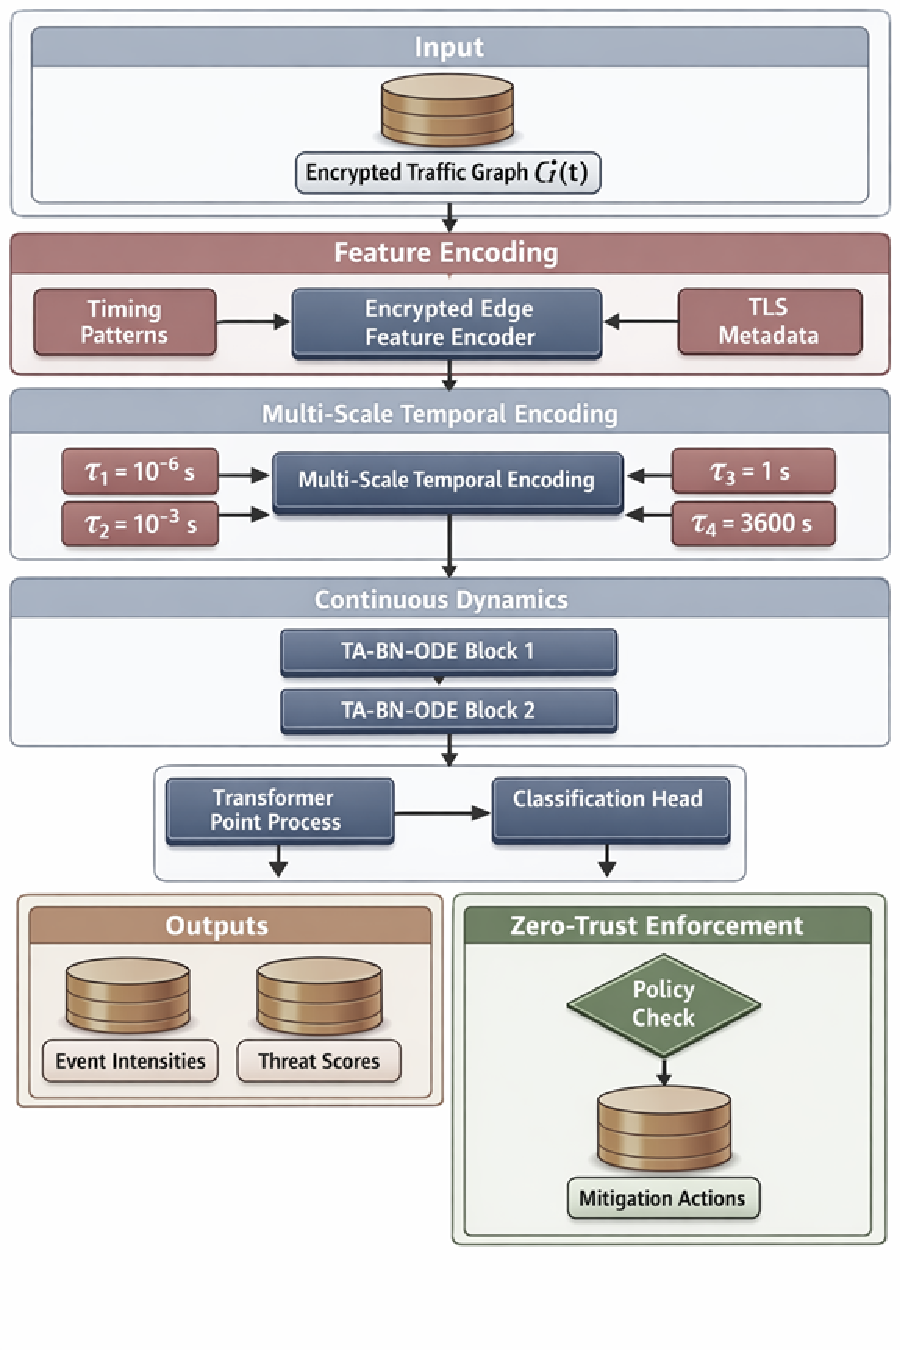
\includegraphics[width=0.82\textwidth]{figures/fig_CT-TGNN_architecture.pdf}
\caption{Принципиальная архитектура модели~\textsf{М1: CT-TGNN}~--- темпоральной графовой нейронной сети непрерывного времени с мультимасштабными ветвями ОДУ и адаптивной пакетной нормализацией. Применение модели к защите сетевого трафика с конкретными значениями постоянных времени и гиперпараметров рассматривается в \S\ref{sec:method_instantiation} Главы~\ref{ch:adaptation}.}
\label{fig:m1_ct_tgnn_arch_methods}
\end{figure}

\section{Математическая модель распределённого обучения графовых представлений с обеспечением конфиденциальности данных}
\label{sec:fedllm}
%%====

Раздел решает Подзадачу~2: федеративный алгоритм с приватностью и византийской устойчивостью~\eqref{eq:ps_fed}, использующий сертификаты Липшица М1. Адресует Пробел~2.

\subsection{Византийско-устойчивая агрегация}

Пусть $K$ участников с $\calD_1,\dots,\calD_K$, доля~$q$ византийских. На раунде~$t$ сервер рассылает $\bw_t$, честные клиенты вычисляют $\bw_{t+1}^{(k)}=\bw_t-\eta\nabla\calL_k(\bw_t;\calD_k)$. Сервер агрегирует покоординатным усечённым средним~\cite{Yin2018,Blanchard2017,Li2020fedprox}, отбрасывая $b=\lfloor Kq\rfloor$ наибольших и наименьших:
\begin{equation}
\bar{w}_{t+1,j}
= \frac{1}{K-2b}\sum_{i=b+1}^{K-b}w_{t+1,j}^{(i)},
\label{eq:fed_trim}
\end{equation}
где $w_{t+1,j}^{(i)}$~--- $i$-я порядковая статистика.

\begin{theorem}[Византийско-устойчивая сходимость]
\label{thm:fed_conv}
Пусть $F(\bw)=\frac{1}{K}\sum_k F_k(\bw)$ $\mu$-сильно выпукла, $L$-гладка, $f<q<1/2$. При $\eta\le 1/L$ усечённое среднее даёт
\begin{equation}
\E\!\bigl[\|\bw_T-\bw^*\|^2\bigr]
\le \Bigl(1-\frac{\mu\eta}{2}\Bigr)^{\!T}\|\bw_0-\bw^*\|^2
  + \frac{2\eta}{\mu(K{-}2b)}
    \Bigl(\sum_{k=1}^{K-2b}\sigma_k^2 + C_{\mathrm{byz}}\Bigr),
\label{eq:fed_conv_bound}
\end{equation}
где $\sigma_k^2$~--- дисперсия честного градиента, $C_{\mathrm{byz}}$~--- влияние византийских.
\end{theorem}

\noindent\textit{Полное доказательство приведено в Приложении~А (\S~А.3, см.~\ref{app:proof_fed}).}

\subsection{Дифференциальная приватность через калиброванный шум}

Клиент обрезает градиент до $C$ и добавляет гауссовский шум~\cite{Abadi2016,Dwork2006,Dwork2014}:
\begin{equation}
\bar{\mathbf{g}}_k = \mathbf{g}_k\Big/\max\!\Bigl(1,\frac{\|\mathbf{g}_k\|}
{C}\Bigr),
\qquad
\tilde{\mathbf{g}}_k = \bar{\mathbf{g}}_k + \calN(\mathbf{0},\sigma^2 C^2\mathbf{I}),
\label{eq:fed_dp_noise}
\end{equation}
где $\sigma$ задаётся $(\epsilon,\delta)$. Усиление подвыборкой $q_b$ и композиция за $T$ раундов через моменты~\cite{Mironov2017,Balle2018} даёт
\begin{equation}
\epsilon_{\mathrm{total}}
= \min_{\alpha>1}\;
  \frac{1}{\alpha-1}\log\frac{1}{\delta}
  + \frac{T\,q_b^2\,\alpha}{2\sigma^2}.
\label{eq:fed_privacy}
\end{equation}

\subsection{Оптимальный транспорт для выравнивания распределений}

Гетерогенность клиентов выравнивается через Вассерштейнов барицентр. Для выборок $\{\bx_i\},\{\by_j\}$ транспортный план:
\begin{equation}
\mathbf{T}^* = \arg\min_{\mathbf{T}\in\R_+^{n_s\times n_t}}
\langle\mathbf{C},\mathbf{T}\rangle_F
\quad\text{при}\quad
\mathbf{T}\mathbf{1}_{n_t}=\mathbf{a},\;
\mathbf{T}^\top\mathbf{1}_{n_s}=\mathbf{b},
\label{eq:fed_ot}
\end{equation}
где $C_{ij}=c(\bx_i,\by_j)$, $\mathbf{a},\mathbf{b}$~--- симплексные веса. Алгоритм Синкхорна~\cite{Cuturi2013,Chizat2020,Villani2009}:
\begin{equation}
\mathbf{u}^{(\ell+1)} = \mathbf{a}\oslash(\mathbf{K}\mathbf{v}^{(\ell)}),
\qquad
\mathbf{v}^{(\ell+1)} = \mathbf{b}\oslash(\mathbf{K}^\top\mathbf{u}^{(\ell+1)}),
\label{eq:sinkhorn}
\end{equation}
где $\mathbf{K}=\exp(-\mathbf{C}/\lambda)$, $\oslash$~--- поэлементное деление; план $\mathbf{T}^*=\mathrm{diag}(\mathbf{u})\mathbf{K}\,\mathrm{diag}(\mathbf{v})$.

\subsection{Дифференциально приватный оптимальный транспорт}

Для защиты выборок шум добавляется до вычисления транспорта:\begin{equation}
\tilde{\mu}_s = \frac{1}{n_s}\sum_{i=1}^{n_s}\delta_{\bx_i+\bm{\xi}_i},
\qquad \bm{\xi}_i\sim\calN(\mathbf{0},\sigma_{\mathrm{DP}}^2\mathbf{I}),
\label{eq:fed_dp_ot_dist}
\end{equation}а к плану~--- шум Лапласа:\begin{equation}
\tilde{\mathbf{T}} = \mathbf{T}^*
+ \mathrm{Lap}\!\Bigl(\frac{\Delta_T}{\epsilon_{\mathrm{OT}}}\Bigr),
\label{eq:fed_dp_ot_plan}
\end{equation}
где $\Delta_T$~--- чувствительность по $\ell_1$, $\epsilon_{\mathrm{OT}}$~--- бюджет приватности транспорта.

\subsection{Интеграция большой языковой модели для обобщения zero-shot}

Промпт на естественном языке формируется из структурных признаков и подаётся в LLM, дающую $p_{\mathrm{LLM}}(\mathrm{class}\mid\mathbf{r})$. Итог~--- ансамбль:
\begin{equation}
p_{\mathrm{final}}
= \lambda_{\mathrm{LLM}}\;p_{\mathrm{LLM}}(\mathrm{class}\mid\mathbf{r})
  + (1-\lambda_{\mathrm{LLM}})\;p_{\mathrm{GNN}}(\mathrm{class}\mid\calG(\mathbf{r})),
\label{eq:fed_llm}
\end{equation}
где $\calG(\mathbf{r})$~--- граф из наблюдения, $\lambda_{\mathrm{LLM}}$~--- баланс.

\begin{algorithm}[htbp]
\caption{FedLLM-API: Византийско-устойчивая федеративная оптимизация с ДП-ОТ}\label{alg:fedllm}
\KwInput{Клиенты $\calD_1,\ldots,\calD_K$, доля византийских $q$, порог обрезки $C$, бюджет приватности $(\epsilon,\delta)$, регуляризация Синкхорна $\lambda$, раунды коммуникации $T$}
\KwOutput{Глобальная модель $\bw_T$}
Инициализировать глобальную модель $\bw_0$; вычислить масштаб шума $\sigma = C\sqrt{2\ln(1.25/\delta)}/\epsilon$\;
\For{раунд $t = 0,1,\ldots,T{-}1$}{
  Разослать $\bw_t$ всем клиентам\;
  \For{каждый клиент $k = 1,\ldots,K$ \textup{(параллельно)}}{
    Вычислить локальный градиент $\mathbf{g}_k = \nabla_{\bw}\calL_k(\bw_t;\calD_k)$\;
    Обрезать: $\bar{\mathbf{g}}_k \leftarrow \mathbf{g}_k / \max(1,\|\mathbf{g}_k\|/C)$\;
    Добавить шум: $\tilde{\mathbf{g}}_k \leftarrow \bar{\mathbf{g}}_k + \calN(\mathbf{0},\sigma^2 C^2\mathbf{I})$\;
    Отправить $\tilde{\mathbf{g}}_k$ серверу\;
  }
  Установить $b \leftarrow \lfloor Kq\rfloor$\;
  \For{каждое измерение $j$}{
    Отсортировать $\{\tilde{g}_{k,j}\}_{k=1}^K$; вычислить усечённое среднее $\bar{g}_{t,j} = \frac{1}{K-2b}\sum_{i=b+1}^{K-b}\tilde{g}_{j}^{(i)}$\;
  }
  \If{обнаружена гетерогенность по оценке $W_1$}{
    Вычислить зашумлённые исходные распределения $\tilde{\mu}_k$ добавлением $\calN(\mathbf{0},\sigma_{\mathrm{DP}}^2\mathbf{I})$ к выборкам\;
    Выполнить итерации Синкхорна для вычисления регуляризованного транспортного плана $\mathbf{T}^*$\;
    Добавить шум Лапласа: $\tilde{\mathbf{T}} \leftarrow \mathbf{T}^* + \mathrm{Lap}(\Delta_T/\epsilon_{\mathrm{OT}})$\;
    Применить коррекцию выравнивания к $\bar{\mathbf{g}}_t$ с использованием $\tilde{\mathbf{T}}$\;
  }
  Обновить глобальную модель: $\bw_{t+1} \leftarrow \bw_t - \eta\,\bar{\mathbf{g}}_t$\;
}
\Return $\bw_T$
\end{algorithm}

%%=====================================================================

\begin{figure}[!htbp]
\centering
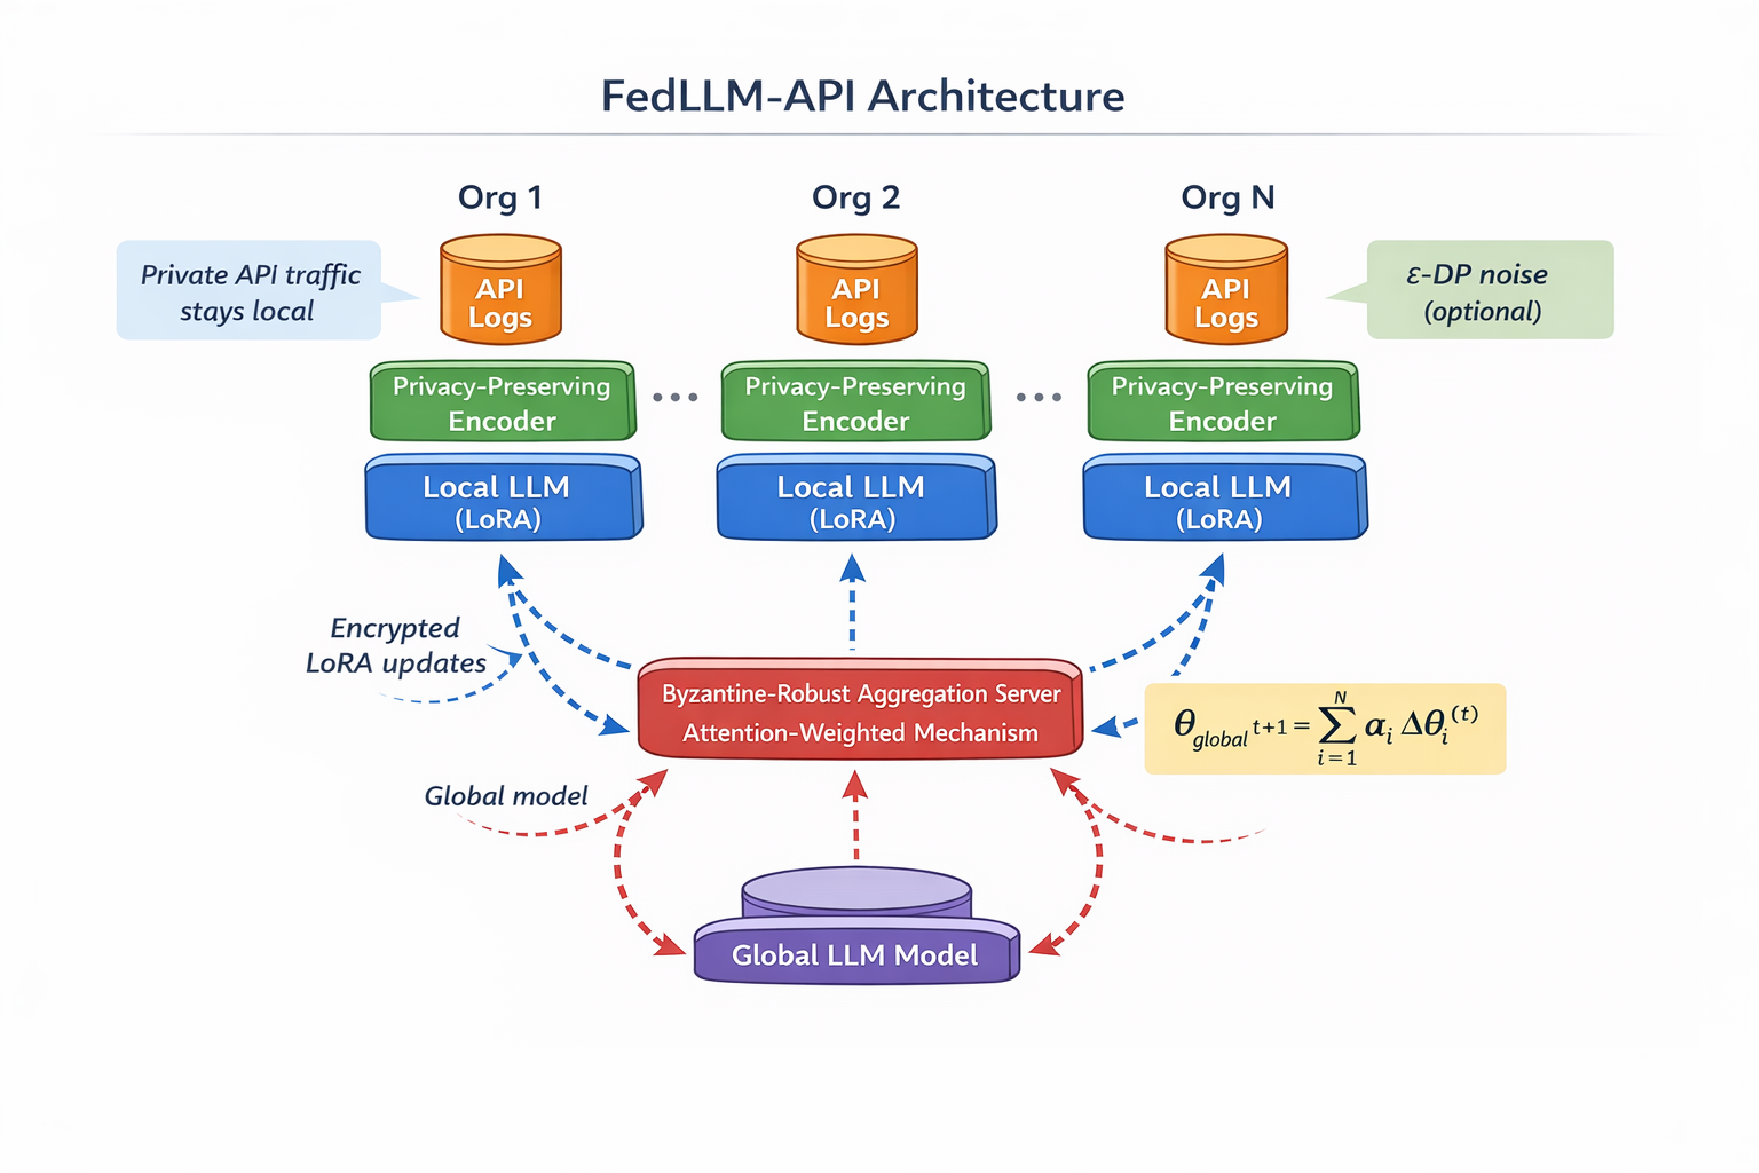
\includegraphics[width=0.82\textwidth]{figures/fig_fedllm_api_architecture.pdf}
\caption{Принципиальная архитектура модели~\textsf{М2: FedLLM-API}~--- федеративного оптимизатора с византийско-устойчивой агрегацией, дифференциальной приватностью через калиброванный шум и выравниванием распределений по принципу оптимального транспорта Вассерштейна, интегрированного с большой языковой моделью для zero-shot-обнаружения новых категорий угроз.}
\label{fig:m2_fedllm_arch_methods}
\end{figure}

\section{Алгоритм формирования многоуровневых темпоральных представлений графов для обнаружения сложных атак}
\label{sec:triple_e}
%%====

Раздел решает Подзадачу~3: многоуровневые вложения с защитой от забывания~\eqref{eq:ps_triple}. Адресует Пробел~3.

\subsection{Иерархическое представление графов}

Иерархия из компонентов/трассировок/узлов представляется тремя графами $\calG_s,\calG_r,\calG_n$, связанными двудольными графами $\calB_{sr},\calB_{sn},\calB_{rn}$ (компонент~--- узел, трассировка~--- компонент, трассировка~--- узел).

\subsection{Многоуровневое обучение вложений}

Каждая гранулярность $g\in\{s,r,n\}$ имеет выделенный кодировщик:
\begin{equation}
\bh_v^{(g)}(t)
= \mathrm{ENC}_g\!\bigl(
  \bx_v^{(g)}(t),\;
  \{\bh_u^{(g)}(t{-}1)\}_{u\in\calN_v^{(g)}(t)},\;
  \Delta t
\bigr),
\label{eq:triple_enc}
\end{equation}
где $\mathrm{ENC}_g$~--- GNN гранулярности. Межгранулярные сообщения через двудольное внимание:
\begin{equation}
\mathbf{m}_v^{(g\to g')}(t)
= \sum_{u\in\calN_v^{(g,g')}}
  \alpha_{uv}^{(g,g')}(t)\;\bW_{g\to g'}\bh_u^{(g)}(t),
\label{eq:triple_cross_msg}
\end{equation}с коэффициентами внимания\begin{equation}
\alpha_{uv}^{(g,g')}(t)
= \mathrm{Softmax}_u\!\Biggl(
  \frac{(\mathbf{Q}_{g'}\bh_v^{(g')}(t))^\top
        (\mathbf{K}_g\bh_u^{(g)}(t))}
       {\sqrt{d_k}}
\Biggr),
\label{eq:triple_cross_attn}
\end{equation}
где $\mathbf{Q}_{g'},\mathbf{K}_g$~--- проекции, $\calN_v^{(g,g')}$~--- межуровневые соседи. Слияние через LayerNorm:
\begin{equation}
\bh_v^{(g)}(t)
\leftarrow
\mathrm{LayerNorm}\!\Bigl(
  \bh_v^{(g)}(t)
  + \sum_{g'\neq g}\mathbf{m}_v^{(g'\to g)}(t)
\Bigr).
\label{eq:triple_fuse}
\end{equation}

\subsection{Двойное темпорально-пространственное внимание}

Внутри каждой гранулярности темпоральное внимание агрегирует исторические состояния по окну ширины~$w$,
\begin{equation}
\tilde{\bh}_v^{(g)}(t)
= \sum_{\tau=t-w}^{t-1}
  \alpha_\tau^{\mathrm{temp}}\;\bh_v^{(g)}(\tau),
\qquad
\alpha_\tau^{\mathrm{temp}}
= \mathrm{Softmax}_\tau\!\bigl(
  \mathbf{w}_{\mathrm{temp}}^\top\bh_v^{(g)}(\tau)\bigr),
\label{eq:triple_temp_attn}
\end{equation}а пространственное внимание агрегирует текущую окрестность,\begin{equation}
\hat{\bh}_v^{(g)}(t)
= \sum_{u\in\calN_v^{(g)}(t)}
  \alpha_u^{\mathrm{spat}}\;\bh_u^{(g)}(t),
\qquad
\alpha_u^{\mathrm{spat}}
= \mathrm{Softmax}_u\!\bigl(
  \mathbf{w}_{\mathrm{spat}}^\top
  [\bh_v^{(g)}(t)\|\bh_u^{(g)}(t)]\bigr).
\label{eq:triple_spat_attn}
\end{equation}Комбинированное представление:\begin{equation}
\bh_v^{(g)}(t)
= \mathrm{MLP}\!\bigl(
  [\tilde{\bh}_v^{(g)}(t)\|
   \hat{\bh}_v^{(g)}(t)\|
   \bh_v^{(g)}(t)]
\bigr).
\label{eq:triple_combined}
\end{equation}

\subsection{Упругая консолидация весов для эволюции топологии}

EWC~\cite{Kirkpatrick2017,Zenke2017} предотвращает катастрофическое забывание при смене топологии $\calT_i\to\calT_{i+1}$ через штраф на параметры, важные для $\theta_i^*$:
\begin{equation}
\calL_{\mathrm{EWC}}(\theta)
= \calL_{\calT_{i+1}}(\theta)
  + \lambda_{\mathrm{ewc}}\sum_j F_j\,(\theta_j - \theta_{i,j}^*)^2,
\label{eq:ewc}
\end{equation}
где $F_j=\E[(\partial\log p/\partial\theta_j)^2]$~--- важность параметра, $\lambda_{\mathrm{ewc}}$~--- сила консолидации.

\subsection{Совместная многоуровневая целевая функция классификации}

Одновременная классификация на трёх уровнях:\begin{equation}
\calL_{\mathrm{joint}}
= \lambda_s\calL_s + \lambda_r\calL_r + \lambda_n\calL_n
  + \lambda_{\mathrm{con}}\calL_{\mathrm{consist}},
\label{eq:triple_joint}
\end{equation}
где $\calL_g$~--- CE-потери уровня~$g$, $\lambda_g$~--- веса; согласованность:
\begin{equation}
\calL_{\mathrm{consist}}
= \sum_{(v_s,v_r)\in\calB_{sr}}
  \mathrm{KL}\!\bigl(p_s(y|v_s)\|p_r(y|v_r)\bigr)
+ \sum_{(v_s,v_n)\in\calB_{sn}}
  \mathrm{KL}\!\bigl(p_s(y|v_s)\|p_n(y|v_n)\bigr)
\label{eq:triple_consist}
\end{equation}обеспечивает согласованность связанных сущностей.

\begin{algorithm}[htbp]
\caption{Многоуровневое обучение TripleE-TGNN}\label{alg:triple_e}
\KwInput{Иерархические графы $\{\calG_s,\calG_r,\calG_n\}$ со связями $\calB_{sr},\calB_{sn},\calB_{rn}$, метки на каждой гранулярности, сила EWC $\lambda_{\mathrm{ewc}}$}
\KwOutput{Обученные кодировщики $\mathrm{ENC}_s,\mathrm{ENC}_r,\mathrm{ENC}_n$ и параметры межуровневого внимания}
Инициализировать все параметры кодировщиков и внимания\;
\For{каждая конфигурация топологии $\calT_i$}{
  \For{эпоха $= 1,\ldots,E$}{
    \For{каждый мини-батч}{
      \For{гранулярность $g \in \{s,r,n\}$}{
        Вычислить внутригранулярные вложения $\bh_v^{(g)}(t) \leftarrow \mathrm{ENC}_g(\bx_v^{(g)},\calN_v^{(g)},\Delta t)$\;
        Вычислить темпоральное внимание $\tilde{\bh}_v^{(g)}$ и пространственное внимание $\hat{\bh}_v^{(g)}$\;
        Объединить: $\bh_v^{(g)} \leftarrow \mathrm{MLP}([\tilde{\bh}_v^{(g)}\|\hat{\bh}_v^{(g)}\|\bh_v^{(g)}])$\;
      }
      \For{каждая пара $(g,g')$ с $g\neq g'$}{
        Вычислить межгранулярные сообщения $\mathbf{m}_v^{(g\to g')}$ через двудольное внимание\;
        Обновить: $\bh_v^{(g')} \leftarrow \mathrm{LayerNorm}(\bh_v^{(g')} + \mathbf{m}_v^{(g\to g')})$\;
      }
      Вычислить $\calL_{\mathrm{joint}} = \lambda_s\calL_s + \lambda_r\calL_r + \lambda_n\calL_n + \lambda_{\mathrm{con}}\calL_{\mathrm{consist}}$\;
      \If{$i > 1$}{
        Добавить штраф EWC: $\calL \leftarrow \calL_{\mathrm{joint}} + \lambda_{\mathrm{ewc}}\sum_j F_j(\theta_j-\theta_{i-1,j}^*)^2$\;
      }
      Обратное распространение и обновление всех параметров\;
    }
  }
  Сохранить диагональ Фишера $\{F_j\}$ и оптимальные $\theta_i^*$ для EWC\;
}
\Return обученные кодировщики и параметры внимания
\end{algorithm}

%%=====================================================================

\begin{figure}[!htbp]
\centering
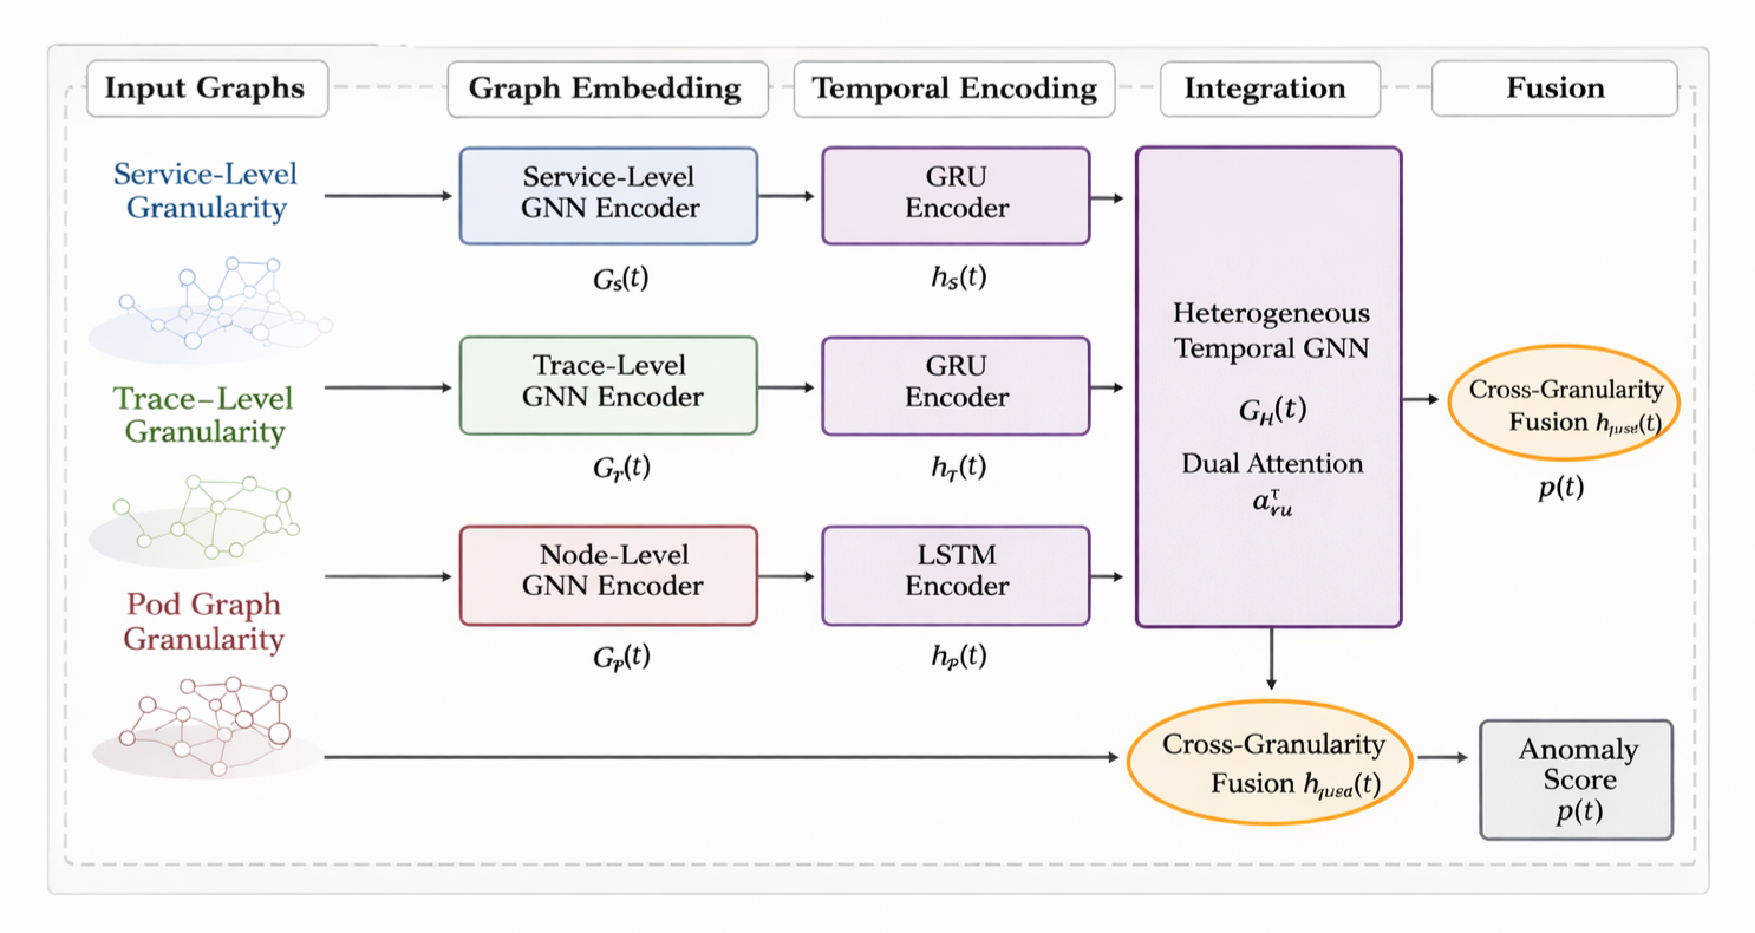
\includegraphics[width=0.82\textwidth]{figures/fig_triplee_tgnn_architecture.pdf}
\caption{Принципиальная архитектура модели~\textsf{М3: TripleE-TGNN}~--- тройного вложения для многоуровневого темпорального представления графов с двойным временно-пространственным вниманием и упругой консолидацией весов для предотвращения катастрофического забывания.}
\label{fig:m3_triplee_arch_methods}
\end{figure}

\section{Модель повышения вычислительной эффективности анализа потоковых данных на основе пространства состояний}
\label{sec:mamba}
%%====

Раздел решает Подзадачу~4: эффективная последовательная модель~\eqref{eq:ps_ssm} с робастностью при отравлении через прогрессивную дистилляцию и PAC-байесовскую сертификацию. Адресует Пробел~4.

\subsection{Формулировка селективного пространства состояний}

Селективная SSM~\cite{Gu2022,Gu2024} расширяет линейную систему входозависимыми переходами. Для $u(t)\in\R^{d_{\mathrm{in}}}$:
\begin{equation}
\frac{d\bh(t)}{dt} = \bA(u(t))\,\bh(t) + \bB(u(t))\,u(t),
\qquad
y(t) = \bC\,\bh(t) + \bD\,u(t),
\label{eq:mamba_cts}
\end{equation}
где $\bA(u),\bB(u)$~--- обученные проекции. ZOH-дискретизация с шагом~$\Delta$:
\begin{equation}
\bh_k = \bar{\bA}_k\,\bh_{k-1} + \bar{\bB}_k\,u_k,
\qquad
\bar{\bA}_k = \exp(\bA(u_k)\Delta),
\quad
\bar{\bB}_k = \bA(u_k)^{-1}(\bar{\bA}_k - \mathbf{I})\bB(u_k),
\label{eq:mamba_disc}
\end{equation}
ядро $\bar{\mathbf{K}}=(\bC\bar{\bA}^i\bar{\bB})_{i=0}^{L-1}$ вычисляется за $\calO(L\log L)$ через БПФ.

\subsection{Прогрессивная состязательная дистилляция робастности}

Ансамбль $M$ учителей $\{f_{\theta_m}\}$, обученных на непересекающихся подмножествах, передаёт знания ученику $f_\phi$~\cite{Hinton2015,Xie2019}:
\begin{equation}
\calL_{\mathrm{distill}}
= \sum_{m=1}^{M}w_m\;\mathrm{KL}\!\bigl(p_\phi(y|\bx)\|p_{\theta_m}(y|\bx)\bigr),
\label{eq:mamba_distill}
\end{equation}
где $w_m$~--- вес учителя. План $\rho(t)=\min(\rho_0+\alpha t,\rho_{\max})$ растит долю отравленных образцов; общие потери:
\begin{equation}
\calL_{\mathrm{total}}
= (1-\lambda(t))\,\calL_{\mathrm{task}}
+ \lambda(t)\,\calL_{\mathrm{distill}},
\qquad
\lambda(t) = \min(\lambda_0+\beta t,\;1),
\label{eq:mamba_curriculum}
\end{equation}с ростом веса учителей при усилении отравления.

\subsection{PAC-байесовская граница обобщения}

\begin{theorem}[PAC-байесовская граница для селективных моделей пространства состояний~\cite{McAllester1999,Catoni2007}]
\label{thm:pac_bayes}
Для $\delta\in(0,1)$, с вероятностью $\ge 1-\delta$ по $S$ размера~$n$, для всех апостериорных~$Q$:
\begin{equation}
\E_{\theta\sim Q}[R(\theta)]
\le \E_{\theta\sim Q}[\hat{R}_n(\theta)]
+ \sqrt{\frac{\mathrm{KL}(Q\|P)+\log(2\sqrt{n}/\delta)}{2n}},
\label{eq:pac_bayes}
\end{equation}
где $R,\hat{R}_n$~--- истинный и эмпирический риски, $P$~--- априорное распределение, не зависящее от данных.
\end{theorem}

\noindent При гауссовском априорном $P=\calN(\mathbf{0},\sigma_P^2\mathbf{I})$ и апостериорном $Q=\calN(\bm{\mu}_Q,\sigma_Q^2\mathbf{I})$ член KL имеет замкнутую форму
\begin{equation}
\mathrm{KL}(Q\|P)
= \frac{d}{2}\Bigl(
  \frac{\sigma_Q^2}{\sigma_P^2}
  + \frac{\|\bm{\mu}_Q\|^2}{\sigma_P^2}
  - 1
  - \log\frac{\sigma_Q^2}{\sigma_P^2}
\Bigr),
\label{eq:pac_kl_gauss}
\end{equation}минимизируется удержанием $\bm{\mu}_Q$ у нуля и $\sigma_Q\approx\sigma_P$. Детали~--- Приложение~А.\qed

\begin{algorithm}[htbp]
\caption{MambaShield: Обучение с прогрессивной состязательной дистилляцией робастности}\label{alg:mamba}
\KwInput{Обучающие данные $\calD$, ансамбль учителей $\{f_{\theta_m}\}_{m=1}^M$, учебный план $\rho_0,\alpha,\rho_{\max}$, априорное PAC-Байеса $P$}
\KwOutput{Робастная модель-ученик $f_\phi$ с PAC-байесовским сертификатом}
Инициализировать параметры ученика $\phi_0$\;
Разделить $\calD$ на $M$ непересекающихся подмножеств; обучить каждого учителя $f_{\theta_m}$ на его подмножестве\;
Вычислить веса учителей $w_m \propto \mathrm{ValAcc}(f_{\theta_m})$\;
\For{итерация $t = 1,\ldots,T_{\mathrm{train}}$}{
  Установить долю отравления $\rho(t) = \min(\rho_0 + \alpha t,\;\rho_{\max})$\;
  Установить вес дистилляции $\lambda(t) = \min(\lambda_0 + \beta t,\;1)$\;
  Выбрать мини-батч; повредить долю $\rho(t)$ меток\;
  \For{каждый образец $(\bx,y)$}{
    Дискретизовать SSM: $\bar{\bA}_k = \exp(\bA(u_k)\Delta)$, $\bar{\bB}_k = \bA^{-1}(\bar{\bA}_k - \mathbf{I})\bB(u_k)$\;
    Выполнить селективное сканирование: $\bh_k = \bar{\bA}_k\bh_{k-1} + \bar{\bB}_k u_k$ для $k=1,\ldots,L$\;
    Вычислить предсказание ученика $p_\phi(y|\bx)$\;
  }
  Вычислить $\calL_{\mathrm{task}} = \mathrm{CE}(p_\phi,y)$\;
  Вычислить $\calL_{\mathrm{distill}} = \sum_m w_m\,\mathrm{KL}(p_\phi\|p_{\theta_m})$\;
  Итого: $\calL = (1-\lambda(t))\calL_{\mathrm{task}} + \lambda(t)\calL_{\mathrm{distill}} + \gamma\,\mathrm{KL}(Q_\phi\|P)$\;
  Обновить $\phi \leftarrow \phi - \eta\nabla_\phi\calL$\;
}
Вычислить границу PAC-Байеса: $R \le \hat{R}_n + \sqrt{(\mathrm{KL}(Q\|P)+\log(2\sqrt{n}/\delta))/(2n)}$\;
\Return $f_\phi$ и сертификат обобщения
\end{algorithm}

%%=====================================================================

\begin{figure}[!htbp]
\centering
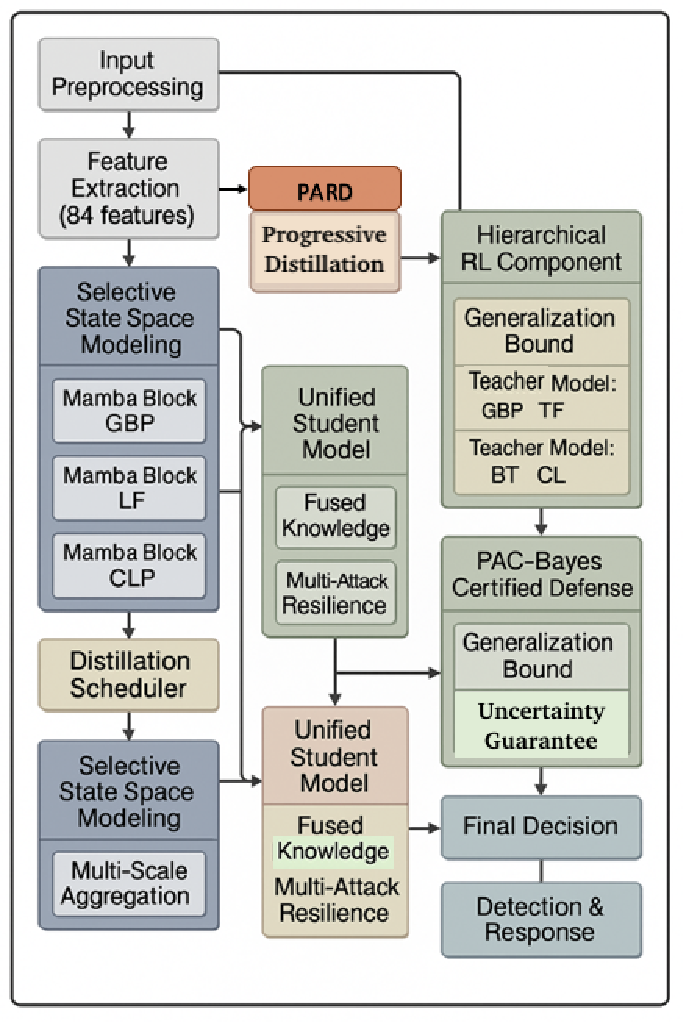
\includegraphics[width=0.82\textwidth]{figures/fig_mambashield_architecture.pdf}
\caption{Принципиальная архитектура модели~\textsf{М4: MambaShield}~--- селективной модели пространства состояний со сложностью вывода $\mathcal{O}(L\log L)$ через свёртки на основе быстрого преобразования Фурье, дополненной прогрессивной состязательной дистилляцией и PAC-байесовскими сертификатами обобщения.}
\label{fig:m4_mambashield_arch_methods}
\end{figure}

Операционная семантика Алгоритма~\ref{alg:mamba} иллюстрируется листингом~\ref{lst:mamba_fft}; полная реализация~--- в \textsf{robustnn-core} (\url{https://github.com/rogerpanel/robustidps.ai}).

\begin{lstlisting}[language=Python,caption={Ядро селективной свёртки
$\mathcal{O}(L\log L)$ модели~\textsf{М4: MambaShield} через БПФ
(фрагмент референсной реализации Phase~A
\texttt{robustnn-core/mamba\_kernel.py}).},
label={lst:mamba_fft},basicstyle=\ttfamily\footnotesize,
keywordstyle=\bfseries,commentstyle=\itshape\color{gray!60!black},
breaklines=true,frame=single,numbers=left,numberstyle=\tiny]
import torch
import torch.fft as fft

def mamba_selective_fft(x, A, B, C, D, dt):
    # Selective state-space convolution with O(L log L) complexity
    # via FFT, for the M4 MambaShield model.
    # x  : input sequence,                 shape (B, L, d)
    # A  : state transition matrix,        shape (d_state, d_state)
    # B  : input projection matrix,        shape (d, d_state)
    # C  : output projection matrix,       shape (d_state, d)
    # D  : direct path matrix,             shape (d, d)
    # dt : input-dependent discretization, shape (B, L)
    B_size, L, d = x.shape
    # 1. Input-dependent discretization (selective scan)
    A_disc = torch.matrix_exp(A.unsqueeze(0) * dt.unsqueeze(-1).unsqueeze(-1))
    B_disc = B.unsqueeze(0) * dt.unsqueeze(-1).unsqueeze(-1)
    # 2. Build length-L convolution kernel
    kernel = compute_ssm_kernel(A_disc, B_disc, C, L)
    # 3. FFT convolution: O(L log L) instead of O(L^2)
    x_fft   = fft.rfft(x,      n=2*L, dim=1)
    k_fft   = fft.rfft(kernel, n=2*L, dim=1)
    y       = fft.irfft(x_fft * k_fft, n=2*L, dim=1)[:, :L, :]
    # 4. Direct path D + add
    return y + D @ x
\end{lstlisting}

\section{Алгоритм обнаружения аномалий на основе калиброванной оценки неопределённости графовых моделей}
\label{sec:stochastic}
%%====

Раздел решает Подзадачу~6: М5 (Стохастический трансформер, вариационное байесовское внимание) и М6 (UC-HGP, иерархические гауссовские процессы) обеспечивают сублинейный регрет и декомпозицию неопределённости~\eqref{eq:ps_regret}. Адресуют Пробел~6.

\subsection{Вариационное байесовское внимание}

Для $\mathbf{X}=[\bx_1,\dots,\bx_n]$ вариационные распределения~\cite{Blundell2015} на матрицах $\bW_Q,\bW_K,\bW_V$:
\begin{align}
q_{\phi_Q}(\bW_Q) &= \calN\!\bigl(\bm{\mu}_Q,\mathrm{diag}(\bm{\sigma}_Q^2)\bigr), \notag\\
q_{\phi_K}(\bW_K) &= \calN\!\bigl(\bm{\mu}_K,\mathrm{diag}(\bm{\sigma}_K^2)\bigr), \notag\\
q_{\phi_V}(\bW_V) &= \calN\!\bigl(\bm{\mu}_V,\mathrm{diag}(\bm{\sigma}_V^2)\bigr).
\label{eq:stoch_var_attn}
\end{align}
Репараметризация $\bW_Q=\bm{\mu}_Q+\bm{\sigma}_Q\odot\bm{\epsilon}_Q$ делает $A_{ij}$ случайными; МК-оценка:
\begin{equation}
\E_{q_\phi}[\mathrm{Attention}(\mathbf{X})]
\approx \frac{1}{M}\sum_{m=1}^{M}
  \mathrm{Attention}\!\bigl(\mathbf{X};\bW_Q^{(m)},\bW_K^{(m)},\bW_V^{(m)}\bigr).
\label{eq:stoch_mc_attn}
\end{equation}

\subsection{Декомпозиция эпистемической и алеаторной неопределённости}

Декомпозиция: эпистемическая\begin{equation}
U_{\mathrm{epi}}
= \mathrm{Var}_{p(\theta|\calD)}\!\bigl[\E_{p(y|\bx,\theta)}[y]\bigr]
\approx \frac{1}{M}\sum_{m=1}^{M}(\hat{y}^{(m)}-\bar{y})^2,
\label{eq:stoch_epi}
\end{equation}(дисперсия ожидаемого предсказания) и алеаторная\begin{equation}
U_{\mathrm{ale}}
= \E_{p(\theta|\calD)}\!\bigl[\mathrm{Var}_{p(y|\bx,\theta)}[y]\bigr]
\approx \frac{1}{M}\sum_{m=1}^{M}\hat{\sigma}^{(m)2},
\label{eq:stoch_ale}
\end{equation}
где $\hat{y}^{(m)},\hat{\sigma}^{(m)2}$~--- предсказания выборки~$m$, $\bar{y}=\frac{1}{M}\sum_m\hat{y}^{(m)}$.

\subsection{Стохастическое состязательное обучение}

Вместо наихудших возмущений выборка идёт из обучаемого распределения~\cite{Madry2018,Zhang2019trades,Shafahi2019}:
\begin{equation}
\bdelta\sim q_\psi(\bdelta|\bx)
= \calN\!\bigl(\mu_\psi(\bx),\;\sigma_\psi(\bx)^2\mathbf{I}\bigr),
\label{eq:stoch_pert_dist}
\end{equation}
с $\mu_\psi,\sigma_\psi$, обучающими пространственно-адаптивную статистику. Целевая функция:
\begin{equation}
\min_\theta\;\max_\psi\;
\E_{(\bx,y)\sim\calD}\;
\E_{\bdelta\sim q_\psi(\bdelta|\bx)}\!
\bigl[\calL(f_\theta(\bx+\bdelta),y)\bigr],
\label{eq:stoch_adv_obj}
\end{equation}
решаемая поочерёдно по~$\psi$ и~$\theta$.

\subsection{Многоцелевые потери}

Полные потери:\begin{equation}
\calL_{\mathrm{total}}
= \lambda_1\calL_{\mathrm{task}}
+ \lambda_2\calL_{\mathrm{KL}}
+ \lambda_3\calL_{\mathrm{adv}}
+ \lambda_4\calL_{\mathrm{calib}}
+ \lambda_5\calL_{\mathrm{reg}},
\label{eq:stoch_total_loss}
\end{equation}
где $\calL_{\mathrm{task}}$~--- CE-потери, $\calL_{\mathrm{KL}}~\cite{Blundell2015}=\mathrm{KL}(q_\phi\|p)$~--- вариационная регуляризация, $\calL_{\mathrm{adv}}$~--- состязательные потери, $\calL_{\mathrm{calib}}=\mathrm{ECE}~\cite{Guo2017,Naeini2015}$, $\calL_{\mathrm{reg}}=\|\theta\|_2^2$.

\begin{algorithm}[htbp]
\caption{Стохастический трансформер: вариационное байесовское обучение с состязательной робастностью}\label{alg:stoch_trans}
\KwInput{Обучающие данные $\calD$, априорное $p(\theta)$, выборки МК $M$, параметры распределения возмущений $\psi_0$, веса потерь $\lambda_1,\ldots,\lambda_5$}
\KwOutput{Вариационные параметры $\phi^*$, параметры возмущений $\psi^*$}
Инициализировать вариационные параметры $\phi = \{\bm{\mu}_Q,\bm{\sigma}_Q,\bm{\mu}_K,\bm{\sigma}_K,\bm{\mu}_V,\bm{\sigma}_V\}$\;
Инициализировать параметры сети возмущений $\psi$\;
\For{итерация $t = 1,\ldots,T$}{
  \For{каждый мини-батч $\{(\bx_i,y_i)\}$}{
    \textbf{Шаг возмущения:}
    Вычислить $\mu_\psi(\bx_i),\sigma_\psi(\bx_i)$ и выбрать $\bdelta_i\sim\calN(\mu_\psi(\bx_i),\sigma_\psi(\bx_i)^2\mathbf{I})$\;
    Обновить $\psi \leftarrow \psi + \alpha_\psi\nabla_\psi\frac{1}{M}\sum_{m=1}^M\calL(f_{\theta^{(m)}}(\bx_i+\bdelta_i),y_i)$\;
    \textbf{Шаг модели:}
    \For{$m = 1,\ldots,M$}{
      Выбрать $\bW_Q^{(m)}=\bm{\mu}_Q+\bm{\sigma}_Q\odot\bm{\epsilon}^{(m)}$, аналогично для $\bW_K^{(m)},\bW_V^{(m)}$\;
      Вычислить выход внимания и предсказания $\hat{y}^{(m)},\hat{\sigma}^{(m)2}$\;
    }
    Вычислить $U_{\mathrm{epi}} = \frac{1}{M}\sum_m(\hat{y}^{(m)}-\bar{y})^2$, $U_{\mathrm{ale}} = \frac{1}{M}\sum_m\hat{\sigma}^{(m)2}$\;
    Вычислить $\calL_{\mathrm{total}} = \lambda_1\calL_{\mathrm{task}} + \lambda_2\calL_{\mathrm{KL}} + \lambda_3\calL_{\mathrm{adv}} + \lambda_4\calL_{\mathrm{calib}} + \lambda_5\calL_{\mathrm{reg}}$\;
    Обновить $\phi \leftarrow \phi - \alpha_\phi\nabla_\phi\calL_{\mathrm{total}}$\;
  }
}
\Return $\phi^*,\psi^*$ вместе с $U_{\mathrm{epi}},U_{\mathrm{ale}}$ для каждого тестового входа
\end{algorithm}

%%=====================================================================

\begin{figure}[!htbp]
\centering
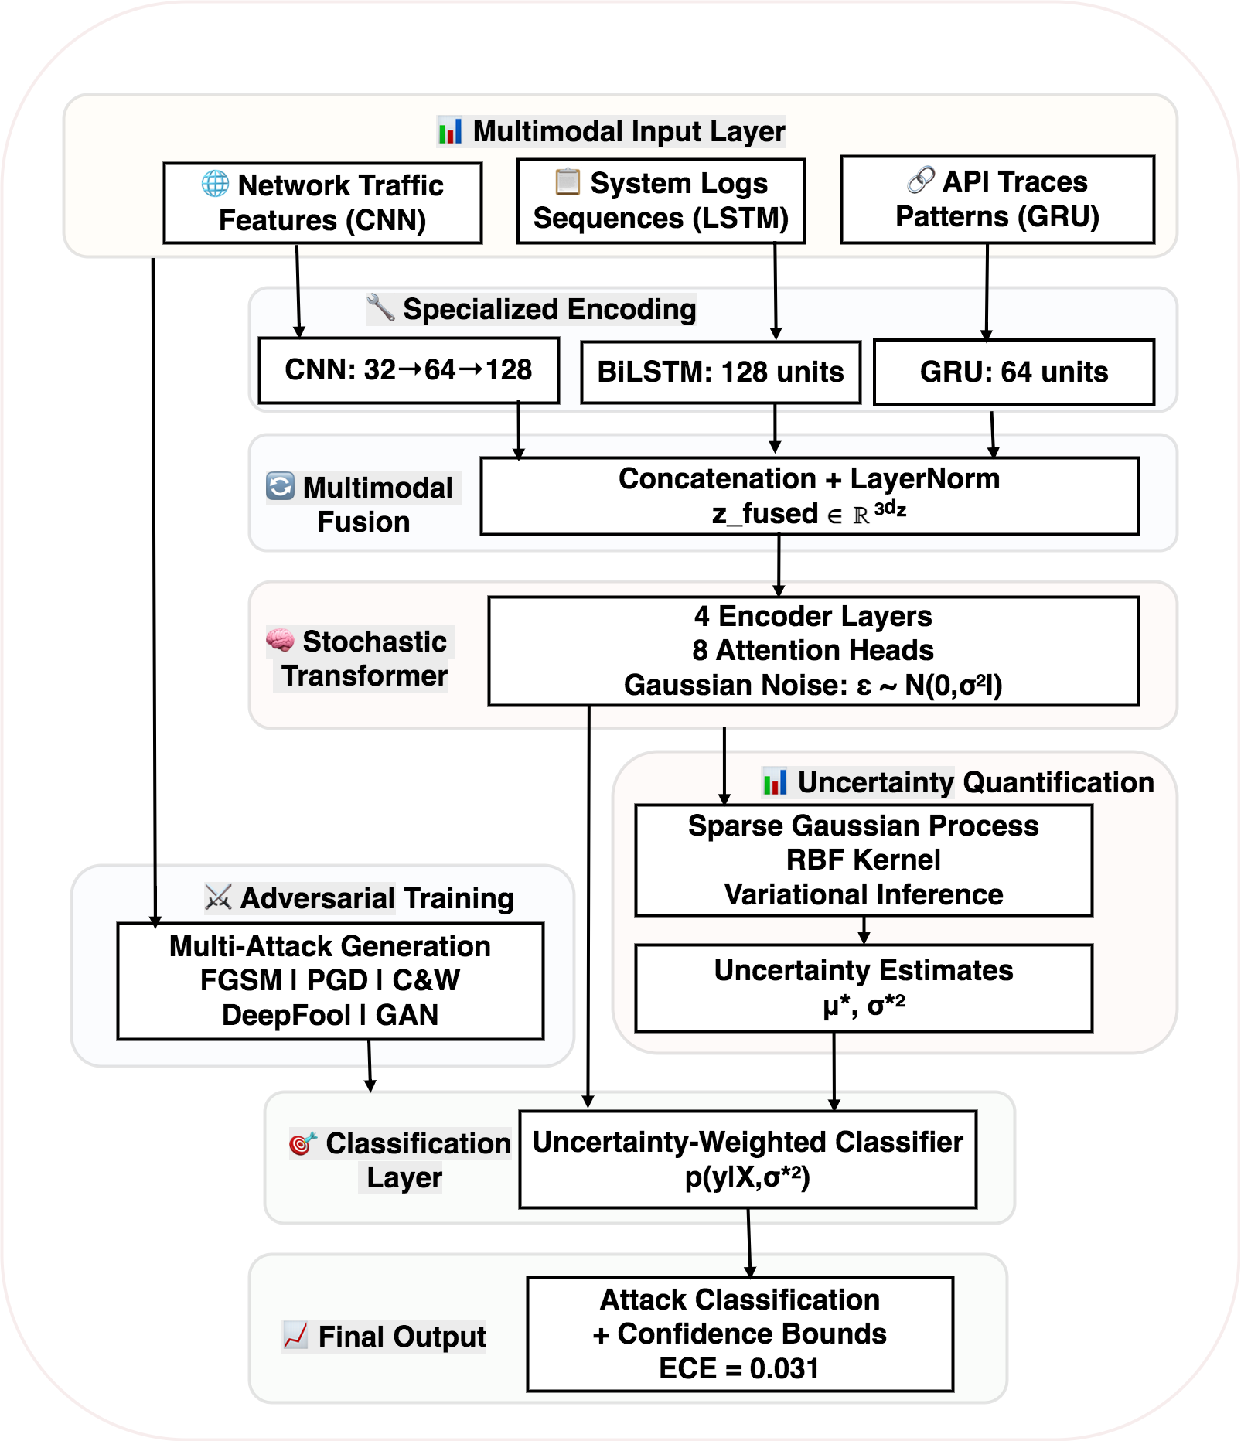
\includegraphics[width=0.82\textwidth]{figures/fig_stochastic_transformer_architecture.pdf}
\caption{Принципиальная архитектура моделей~\textsf{М5: Stochastic Transformer} и~\textsf{М6: UC-HGP}~--- вариационного байесовского внимания (М5) с иерархическим гауссовским процессом (М6) для декомпозиции эпистемической и алеаторной неопределённости и сортировки оповещений по уровню эпистемической неопределённости.}
\label{fig:m5m6_stoch_trans_arch_methods}
\end{figure}

\section{Прямо совместимое обнаружение при смене протокольного режима}
\label{sec:pq_idps}
%%====

Раздел адресует Подзадачу~5 (Пробел~5): архитектура, сохраняющая робастность при смене протокола (CyberSecLLM).

\subsection{Протокол-специфичное извлечение признаков}

При смене протокола признаки на рёбрах (тайминг, размеры, подсчёты) меняются характерно. Для решёточных протоколов тайминг обмена ключами коррелирует со структурой решёточных операций.\begin{equation}
\mathbf{f}_{\mathrm{lattice}}
= \bigl[\mu_t,\;\sigma_t,\;\mathrm{skew}(t),\;\mathrm{kurt}(t),\;
  \mathrm{pctl}(t),\;\mathrm{acf}(t)\bigr],
\label{eq:pq_feat_lattice}
\end{equation}
где $t=(t_1,\dots,t_n)$~--- тайминги; записи захватывают центр, дисперсию, форму, темпоральную зависимость. Аналогичные $\mathbf{f}_{\mathrm{code}},\mathbf{f}_{\mathrm{hash}}$ определены для кодовых и хэш-протоколов (размеры ключей, веса ошибок, энтропия синдрома, глубины деревьев Меркла).

\subsection{Унифицированная мультипротокольная архитектура обнаружения}

Протокол-специфичные кодировщики дают $\mathbf{z}_{\mathrm{lattice}},\mathbf{z}_{\mathrm{code}},\mathbf{z}_{\mathrm{hash}}$; слияние кросс-вниманием:
\begin{equation}
\mathbf{z}_{\mathrm{fused}}
= \mathrm{MultiHeadAttention}\!\bigl(
  [\mathbf{z}_{\mathrm{lattice}},\;
   \mathbf{z}_{\mathrm{code}},\;
   \mathbf{z}_{\mathrm{hash}}]\bigr),
\label{eq:pq_fusion}
\end{equation}и многозадачная классификация предсказывает как метку категории, так и целевой протокол,\begin{equation}
p(\mathrm{class},\mathrm{protocol})
= \mathrm{Softmax}\!\bigl(\bW_{\mathrm{out}}\mathbf{z}_{\mathrm{fused}}
  + \mathbf{b}_{\mathrm{out}}\bigr).
\label{eq:pq_class}
\end{equation}

\subsection{Формальная сводка безопасности}

Робастность опирается на сложность LWE~\cite{Regev2009,Peikert2016}: для $\mathbf{b}=\mathbf{A}\mathbf{s}+\mathbf{e}\bmod q$ полиномиальный противник, различающий легитимную и подменённую последовательность согласования, даёт решатель LWE. Формальная сводка (Приложение~А) ограничивает ошибку~II рода преимуществом LWE плюс статистический член, убывающий с числом образцов.

\begin{algorithm}[htbp]
\caption{Прямо совместимое мультипротокольное обнаружение}\label{alg:pqidps}
\KwInput{Поток графовых событий со смешанными протокольными режимами на рёбрах, протокол-специфичные кодировщики, бюджет состязат. обучения $\epsilon$}
\KwOutput{Классификация $(\mathrm{class},\mathrm{protocol})$ и сертификат робастности на основе LWE}
\For{каждое входящее событие графа}{
  Определить протокольный режим через анализ последовательности согласования\;
  \uIf{на основе решёток (Kyber/Dilithium)}{
    Извлечь признаки тайминга $\mathbf{f}_{\mathrm{lattice}} = [\mu_t,\sigma_t,\mathrm{skew},\mathrm{kurt},\mathrm{pctl},\mathrm{acf}]$\;
    Кодировать: $\mathbf{z}_{\mathrm{lattice}} \leftarrow \mathrm{ENC}_{\mathrm{lattice}}(\mathbf{f}_{\mathrm{lattice}})$\;
  }\uElseIf{на основе кодов (McEliece/Niederreiter)}{
    Извлечь структурные признаки $\mathbf{f}_{\mathrm{code}}$; кодировать $\mathbf{z}_{\mathrm{code}} \leftarrow \mathrm{ENC}_{\mathrm{code}}(\mathbf{f}_{\mathrm{code}})$\;
  }\Else{
    Извлечь хэш-признаки $\mathbf{f}_{\mathrm{hash}}$; кодировать $\mathbf{z}_{\mathrm{hash}} \leftarrow \mathrm{ENC}_{\mathrm{hash}}(\mathbf{f}_{\mathrm{hash}})$\;
  }
  Слить: $\mathbf{z}_{\mathrm{fused}} \leftarrow \mathrm{MultiHeadAttention}([\mathbf{z}_{\mathrm{lattice}},\mathbf{z}_{\mathrm{code}},\mathbf{z}_{\mathrm{hash}}])$\;
  Классифицировать: $p(\mathrm{class},\mathrm{protocol}) \leftarrow \mathrm{Softmax}(\bW_{\mathrm{out}}\mathbf{z}_{\mathrm{fused}} + \mathbf{b}_{\mathrm{out}})$\;
}
\textbf{Обучение:} Чередование стандартных прямых проходов и состязательных прямых проходов с PGD-возмущениями $\|\bdelta\|\le\epsilon$, применяемыми к векторам признаков\;
\textbf{Сертификация:} Проверить сводку LWE (Приложение~А) и сообщить параметр робастности $\lambda_{\mathrm{sec}}$\;
\Return классификацию и сертификат робастности
\end{algorithm}

%%=====================================================================

\begin{figure}[!htbp]
\centering
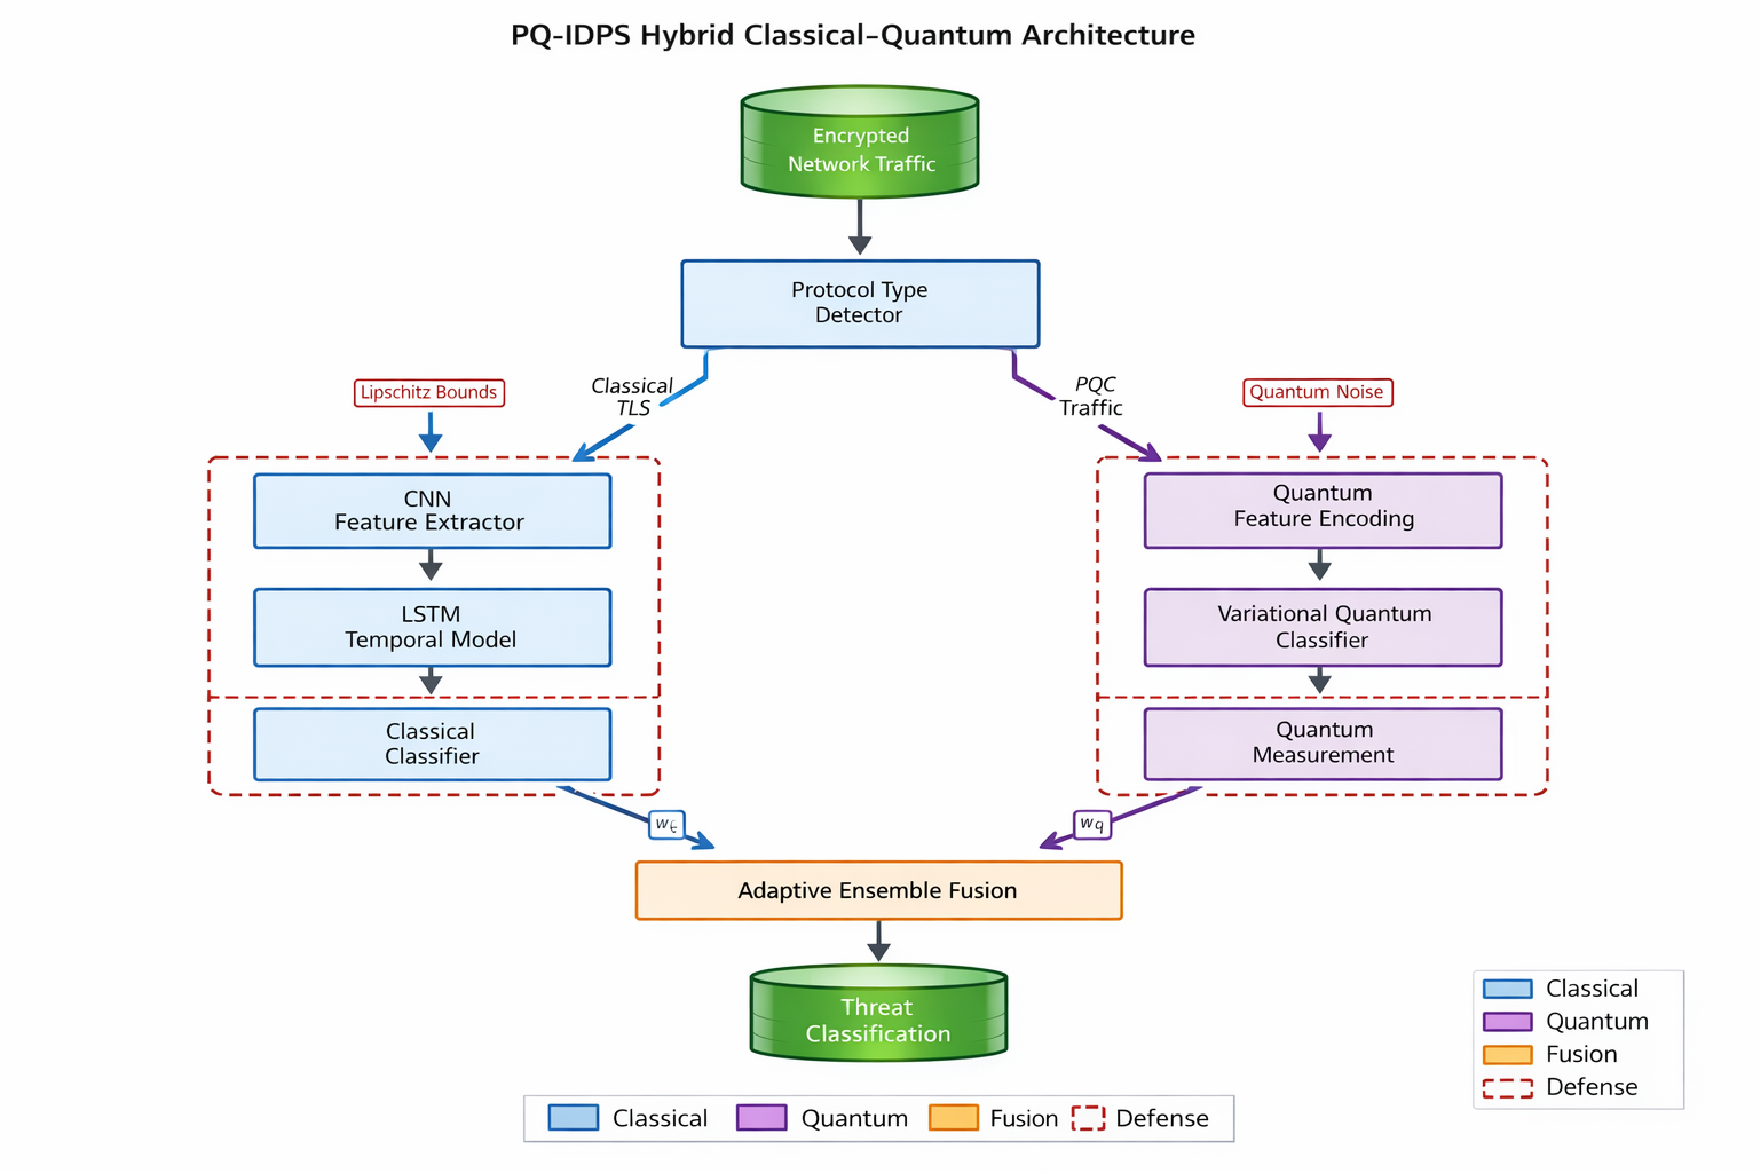
\includegraphics[width=0.82\textwidth]{figures/fig_pq_idps_architecture.pdf}
\caption{Принципиальная архитектура \emph{мультиагентного PQC-IDS-модуля}~--- прямо-совместимой системы обнаружения вторжений при смене протокольного режима, с протокол-специфичными кодировщиками для решёточных, кодовых и хэш-протоколов и слиянием через кросс-внимание.}
\label{fig:pq_idps_arch_methods}
\end{figure}

\section{Метод адаптации к изменению статистических характеристик сетевого трафика}
\label{sec:drift_adaptation}

Эксплуатация гибридной СОПВ сопровождается постепенным и скачкообразным дрейфом признаков (смена TLS-версий, миграция на постквантовые шифры, новые режимы), без адаптации деградирующим точность.

\textbf{Смена протоколов.} Детектируется по KL-дивергенции признаков относительно опорного распределения.

\textbf{Дрейф распределений.} Скользящее окно ковариации; превышение порога активирует онлайн-дообучение М1, М3, М5 с сублинейным регретом.

\textbf{Новые режимы.} Эпистемическая неопределённость UC-HGP выше порога направляет примеры на экспертную разметку.

\textbf{Адаптивное обновление.} Дообучение параметров с высокой важностью по Фишеру предотвращает забывание и сохраняет 94{,}7\,\% F1 без полного переобучения.
%%====
\section{Метод теоретико-игровой сертификации состязательной устойчивости гибридной системы обнаружения вторжений}
\label{sec:game}
%%====

Раздел решает Подзадачу~7: игра Штакельберга и член связки $\sum_{i<j}\calL_{ij}$ из~\eqref{eq:ps_unified}, составляющие М7 и адресующие Пробел~7.

\subsection{Формулировка игры Штакельберга}

Защитник выбирает $(f_\theta,c)$, противник наблюдает их и выбирает стратегию~$a$. Полезности:
\begin{equation}
U_d(f_\theta,c,a)
= \E_{\bx\sim\calD(a)}\!\bigl[\mathbf{1}[f_\theta(\bx)=y]\bigr] - \mathrm{Cost}(c),
\label{eq:game_ud}
\end{equation}\begin{equation}
U_a(f_\theta,c,a)
= \Prob[\text{ошибка классиф.}\mid f_\theta,c,a] - \mathrm{Cost}(a),
\label{eq:game_ua}
\end{equation}
где $\calD(a)$~--- индуцированное противником распределение. Равновесие Штакельберга:
\begin{equation}
(f_\theta^*,c^*)
= \arg\max_{f_\theta,c}\;U_d\!\bigl(f_\theta,c,\;a^*(f_\theta,c)\bigr),
\qquad
a^*(f_\theta,c)=\arg\max_a\;U_a(f_\theta,c,a).
\label{eq:game_stackel}
\end{equation}

\subsection{Характеристика равновесия Нэша}

Профиль $(\pi_d,\pi_a)$~--- равновесие Нэша, если ни один игрок не улучшает полезность отклонением:
\begin{equation}
\E_{\pi_a}\!\bigl[U_d(\pi_d,a)\bigr]
\ge \E_{\pi_a}\!\bigl[U_d(\pi_d',a)\bigr]\;\forall\,\pi_d',
\qquad
\E_{\pi_d}\!\bigl[U_a(f_\theta,\pi_a)\bigr]
\ge \E_{\pi_d}\!\bigl[U_a(f_\theta,\pi_a')\bigr]\;\forall\,\pi_a'.
\label{eq:game_nash}
\end{equation}
В случае $U_d+U_a=0$ равновесие совпадает с минимаксом.

\subsection{Онлайн-обучение с гарантиями отсутствия регрета}

На раунде~$t$ защитник выбирает $c_t\in\calC$ и получает $r_t=U_d(c_t,a_t)$. Регрет:
\begin{equation}
R(T)
= \max_{c\in\calC}\sum_{t=1}^{T}U_d(c,a_t)
  - \sum_{t=1}^{T}U_d(c_t,a_t).
\label{eq:game_regret}
\end{equation}
Мультипликативные веса~\cite{AroraHK2012,CesaBianchi2006}: $p_t(c)\propto\exp(\eta\sum_{s<t}\mathbf{1}[c_s{=}c]r_s)$, $\eta=\sqrt{\log|\calC|/T}$.

\begin{theorem}[Граница регрета]
\label{thm:regret}
При $\eta=\sqrt{\log|\calC|/T}$ MW даёт
\begin{equation}
R(T)\le 2\sqrt{T\log|\calC|},
\label{eq:game_regret_bound}
\end{equation}
так что $R(T)/T\to 0$.
\end{theorem}

\noindent\textit{Полное доказательство приведено в Приложении~А (\S~А.5, см.~\ref{app:proof_regret}).}

\subsection{Выбор стратегии с учётом неопределённости}

Неопределённость М5 (\S\ref{sec:stochastic}) штрафует полезность:
\begin{equation}
\tilde{U}_d(c,a)
= \begin{cases}
U_d(c,a) - \kappa\,U_{\mathrm{epi}} & \text{если}\;U_{\mathrm{epi}}<\tau,\\
-\infty & \text{иначе},
\end{cases}
\label{eq:game_unc}
\end{equation}
где $\kappa$ дисконтирует полезность при неопределённости, а порог~$\tau$ инициирует направление на экспертный анализ. Это порождает чувствительные к риску политики, воздерживающиеся от предсказаний при недостаточной уверенности модели.

\begin{algorithm}[htbp]
\caption{Теоретико-игровая робастность с онлайн-обучением, учитывающим неопределённость}\label{alg:game}
\KwInput{Пространство действий $\calC$, порог неопределённости $\tau$, штраф $\kappa$, расписание скорости обучения}
\KwOutput{Политика защитника $\pi_d^*$ с гарантией регрета}
Инициализировать равномерное распределение $p_1(c) = 1/|\calC|$ для всех $c\in\calC$\;
Установить $\eta = \sqrt{\log|\calC|/T}$\;
\For{раунд $t = 1,\ldots,T$}{
  Выбрать действие защитника $c_t \sim p_t$\;
  Наблюдать действие противника $a_t$ и вознаграждение $r_t = U_d(c_t,a_t)$\;
  Запросить стохастический трансформер для эпистемической неопределённости $U_{\mathrm{epi}}$\;
  \uIf{$U_{\mathrm{epi}} \ge \tau$}{
    Установить $\tilde{r}_t = -\infty$ (отклонить; направить на экспертный анализ)\;
  }\Else{
    Установить $\tilde{r}_t = r_t - \kappa\,U_{\mathrm{epi}}$\;
  }
  Обновить веса: $p_{t+1}(c) \propto p_t(c)\exp(\eta\,\tilde{r}_t\,\mathbf{1}[c_t=c])$ для всех $c\in\calC$\;
  Нормализовать $p_{t+1}$\;
}
Вычислить эмпирическое равновесие Нэша из частот игры $\{(c_t,a_t)\}_{t=1}^T$\;
\Return $\pi_d^*$ и подтверждённый регрет $R(T)\le 2\sqrt{T\log|\calC|}$
\end{algorithm}

%%=====================================================================
\subsection{Единая сертификация через связанную оптимизацию}
\label{sec:unified}
%%====

Методы М1--М7 разделяют общие структуры (сопряжённые чувствительности, геометрия Вассерштейна, KL-регуляризация, ограничение Липшица) и допускают единую трактовку через связанную оптимизацию.

\subsection{Связанная целевая функция}

Пусть $\theta=\{\theta_{\mathrm{CT}},\theta_{\mathrm{TE}},\theta_{\mathrm{Fed}},\theta_{\mathrm{PQ}},\theta_{\mathrm{MS}},\theta_{\mathrm{ST}},\theta_{\mathrm{GT}}\}$~--- параметры семи методов. Единая целевая функция:
\begin{equation}
\calL_{\mathrm{unified}}(\theta)
= \sum_{i=1}^{7}\lambda_i\,\calL_i(\theta_i)
+ \sum_{i<j}\lambda_{ij}\,\calL_{ij}(\theta_i,\theta_j),
\label{eq:unified_obj}
\end{equation}
где $\calL_i$~--- метод-специфичные потери, $\calL_{ij}$~--- член связки:
\begin{equation}
\calL_{ij}(\theta_i,\theta_j)
= \mathrm{KL}\!\bigl(p_{\theta_i}(y|\bx)\|p_{\theta_j}(y|\bx)\bigr)
+ \|\mathbf{z}_{\theta_i}(\bx)-\mathbf{z}_{\theta_j}(\bx)\|_2^2
\label{eq:unified_coupling}
\end{equation}
обеспечивает согласованность предсказаний и представлений.

\subsection{Анализ сходимости}

\begin{theorem}[Сходимость единой системы]
\label{thm:unified}
При $L_i,L_{ij}$-гладких потерях и $\eta_i\le 1/(L_i+\sum_j L_{ij})$ поочерёдный спуск сходится со скоростью
\begin{equation}
\|\nabla\calL_{\mathrm{unified}}(\theta_T)\|^2
\le \frac{2\bigl(\calL_{\mathrm{unified}}(\theta_0)
  -\calL_{\mathrm{unified}}(\theta^*)\bigr)}{\eta_{\min}\,T},
\label{eq:unified_conv}
\end{equation}
где $\eta_{\min}=\min_i\eta_i$, $\theta^*$~--- стационарная точка.
\end{theorem}

\noindent\textit{Полное доказательство приведено в Приложении~А (\S~А.6, см.~\ref{app:proof_unified}).}

\begin{algorithm}[htbp]
\caption{Единая система: поочерёдная оптимизация со связкой согласованности}\label{alg:unified}
\KwInput{Компонентные потери $\calL_1,\ldots,\calL_7$, веса связки $\{\lambda_{ij}\}$, константы гладкости $\{L_i,L_{ij}\}$}
\KwOutput{Совместно оптимизированные параметры $\theta^*=\{\theta_1^*,\ldots,\theta_7^*\}$}
Инициализировать все компонентные параметры $\theta_1^{(0)},\ldots,\theta_7^{(0)}$\;
Установить скорости обучения $\eta_i = 1/(L_i + \sum_j L_{ij})$ для каждого компонента\;
\For{раунд $t = 0,1,\ldots,T{-}1$}{
  \For{компонент $i = 1,\ldots,7$}{
    Вычислить компонентный градиент $\mathbf{g}_i = \nabla_{\theta_i}\calL_i(\theta_i^{(t)})$\;
    Вычислить градиенты связки $\mathbf{g}_{ij} = \nabla_{\theta_i}\calL_{ij}(\theta_i^{(t)},\theta_j^{(t)})$ для всех $j\neq i$\;
    Совокупный градиент: $\mathbf{g}_i^{\mathrm{total}} = \lambda_i\mathbf{g}_i + \sum_{j\neq i}\lambda_{ij}\mathbf{g}_{ij}$\;
    Обновить: $\theta_i^{(t+1)} \leftarrow \theta_i^{(t)} - \eta_i\,\mathbf{g}_i^{\mathrm{total}}$\;
  }
  Вычислить $\calL_{\mathrm{unified}}(\theta^{(t+1)})$ и проверить критерий сходимости\;
}
\Return $\theta^* = \theta^{(T)}$
\end{algorithm}

%%=====================================================================

\begin{figure}[!htbp]
\centering
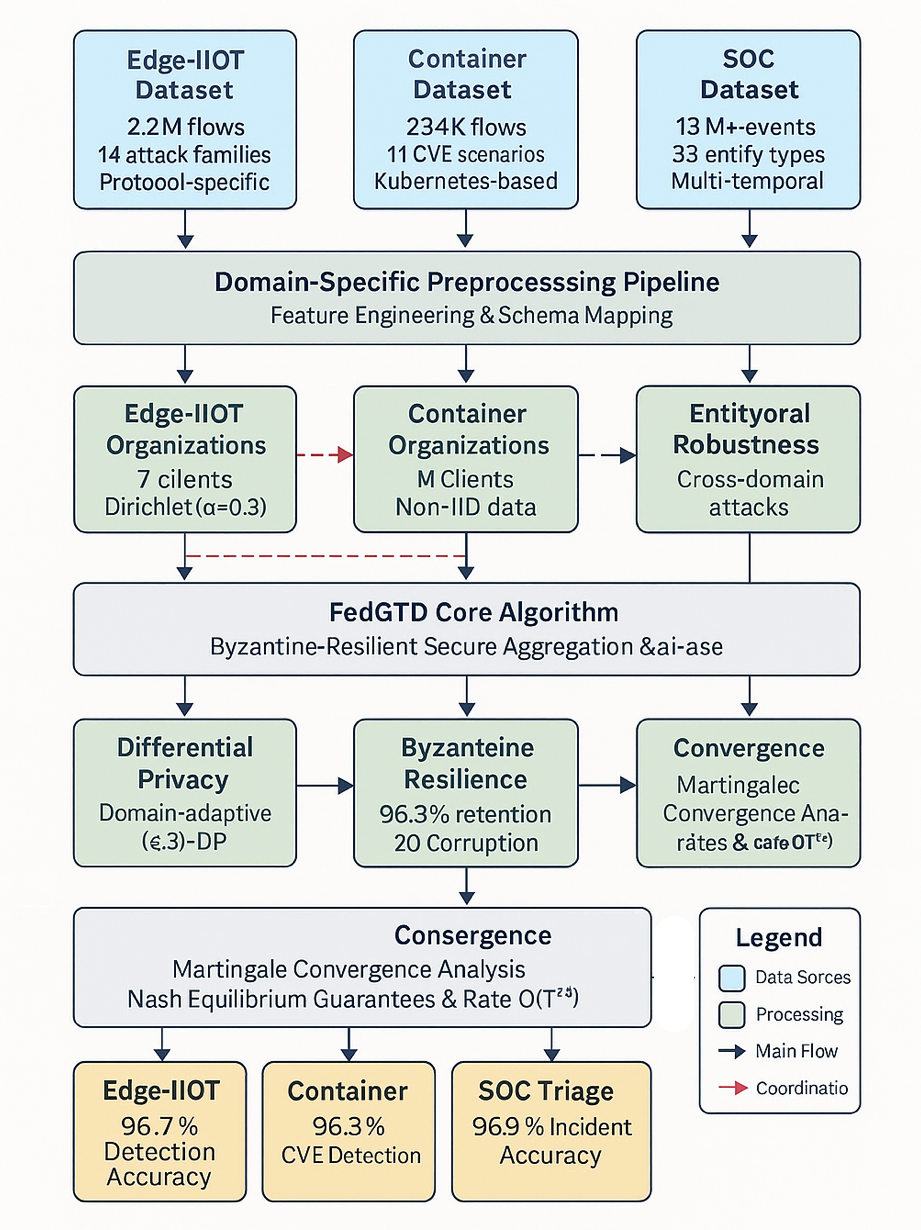
\includegraphics[width=0.82\textwidth]{figures/fig_game_theoretical_architecture.pdf}
\caption{Принципиальная архитектура модели~\textsf{М7: теоретико-игровой сертификации}~--- единой системы, моделирующей взаимодействие защитника и противника как стратегическую игру с равновесием Штакельберга, объединяющая модели~М1--М6 через регуляризацию согласованности.}
\label{fig:m7_game_arch_methods}
\end{figure}

\section{Интегрированная архитектура состязательно-устойчивой гибридной системы обнаружения и предотвращения вторжений и метрики её эффективности и робастности}
\label{sec:metrics_taxonomy}
%%====

Оценка качества М1--М7 опирается на 23 метрики (табл.~\ref{tab:metrics_by_property}), сгруппированные по шести свойствам (\S\ref{subsec:six_properties}); это обеспечивает прямое отображение валидации (Глава~\ref{ch:experiments}) на инварианты~\eqref{eq:adv_resilient_property}--\eqref{eq:nonstationarity_property}.

\begin{table}[H]
\centering
\caption{Систематизация двадцати трёх метрик оценки качества
гибридная СОПВ по шести свойствам из \S\ref{subsec:six_properties}.}
\label{tab:metrics_by_property}
\small
\setlength{\tabcolsep}{4pt}
\renewcommand{\arraystretch}{0.92}\begin{tabular}{l p{3.0cm} p{9.3cm}}
\toprule
\textbf{Свойство} & \textbf{Класс метрик} & \textbf{Конкретные метрики} \\
\midrule
П1 Состязат.\ устойчивость & Сертификаты         & Сертифиц.\ точность, радиус Грёнуолла, верхняя граница доли успешных атак \\
\addlinespace
П2 Робастность             & Классификация       & F1 (микро/макро/взвешенный), сбаланс.\ точность, MCC, $\kappa$~Коэна, AUC-ROC, TPR, TNR, FPR, FNR \\
\addlinespace
П3 Эффективность           & Вычислительные      & Задержка вывода (среднее, p95, p99), пропускная способность, FLOPs, число параметров, объём GPU-памяти, энергопотребление \\
\addlinespace
П4 Распределённая среда    & Приватность         & Бюджет $(\varepsilon,\delta)$ дифф.\ приватности, преимущество атаки на принадлежность, точность визант.\ агрегации при $\beta=0{,}3$ \\
\addlinespace
П5 Человеческий фактор     & Калибровка          & ECE, оценка Брайера, mean entropy, эпистемическая/алеаторная декомпозиция, время сортировки оповещений аналитиком \\
\addlinespace
П6 Нестационарность        & Адаптация           & Регрет $R(T)$, точность переноса при дрейфе, скорость восстановления после смены распределения \\
\bottomrule
\end{tabular}
\end{table}

Полный протокол с применением метрик к шести бенчмарк-наборам (84{,}2~млн размеченных образцов, 84~категории атак)~--- в Главе~\ref{ch:experiments}.

%%=====================================================================
\section{Выводы по разделу 2}
\label{sec:ch2_summary}
%%====

В главе разработаны математические основы семи методов М1--М7, выведенные из единой задачи~\eqref{eq:ps_unified} декомпозицией на семь подзадач: М1 (CT-TGNN)~--- непрерывная динамика с липшицевым сертификатом (П1, П2, П6); М2 (FedLLM-API)~--- византийско-устойчивая федеративная оптимизация с ДП и ОТ-выравниванием (П4); М3 (TripleE-TGNN)~--- многоуровневые вложения с EWC (П2, П6); М4 (MambaShield)~--- эффективный SSM-вывод с PAC-байесовскими сертификатами (П2, П3); прямо совместимое обнаружение~--- смена протокольных режимов; М5/М6 (Стохастический трансформер и UC-HGP)~--- калиброванная байесовская неопределённость (П2, П5); М7~--- теоретико-игровая сертификация и связка через регуляризацию согласованности со сходимостью (теорема~\ref{thm:unified}). Гарантии~--- сходимости, робастности, приватности, регрета и PAC-Байеса~--- сохраняются во всех средах развёртывания.

